\documentclass[11pt,hidelinks]{memoir}

\usepackage{fenna-files/packages}
\addbibresource{fenna-files/references.bib}
\usepackage{fenna-files/abbreviations}

\title{Case competition in headless relatives}
\author{Fenna Bergsma}
\date{\today}

\begin{document}

\bookmarksetup{startatroot}

\frontmatter

\begin{titlingpage}
  \maketitle
\end{titlingpage}

\clearpage
\tableofcontents

\clearpage
\listoftables

\chapter*{List of abbreviations}
\begingroup
  \setlength{\LTleft}{-\tabcolsep}
\printacronyms[include=abbr, heading=none]
\endgroup
\addcontentsline{toc}{chapter}{List of abbreviations}


%%%%
\mainmatter
\setcounter{secnumdepth}{4}

% !TEX root = thesis.tex

\chapter{Introduction}

This dissertation is about case competition, a situation in which two cases are assigned but only one of them surfaces. One of the constructions in which case competition appears is relative clauses that lack a head, i.e. headless relatives.

I show that one aspect about case competition in headless relatives holds for all languages (under discussion here at least). That is, there is a fixed order which decides which case wins the competition. Another aspect of case competition in headless relatives differs per language. That is, whether the competition takes place to begin with. I connect this variable to the morphology of the language in question.

This phenomenon has been described as some special property of a few special languages. Therefore, language-specific rules have been postulated to account for the data. My goal is to show that this phenomenon can be captured with `normal' syntactic processes, like ellipsis, c-command. The account makes predictions about how a language behaves based on the shape of its relative pronouns. And we see that the phenomenon is actually more wide-spread than what has been assumed.
%%this is too difficult

In this introduction I first introduce what I mean exactly with case competition in headless relatives. Then I introduce the topics I discuss in this dissertation.


\section{Introducing the title}

First, case marks the grammatical role of the noun phrases. Case also appears on relative pronoun. Case on head can differ from case on relative pronoun. What happens if there is no noun? Two cases come together on the relative pronoun. What holds for all languages: there is a fixed order of who wins the competition. Specific from language to language: when does the competition take place?

Languages can use case to mark the grammatical role of a noun phrase in a clause. Consider the two Modern German sentences in \ref{ex:germancase}. The case marking of the noun phrases is reflected on the determiner in the noun phrase.
In \ref{ex:germancase1}, \tit{der} in \tit{der Lehrer} `the teacher' is assigned nominative case, because it is the subject in the clause. \tit{Den} in \tit{den Schüler} `the pupil' is assigned accusative case, because it is an object of \tit{mag} `likes'.
In \ref{ex:germancase2}, the roles are reversed: \tit{der} in \tit{der Schüler} `the pupil' is assigned nominative case, because it is the subject in the clause. \tit{Den} in \tit{den Lehrer} `the teacher' is assigned accusative case, because it is the object of \tit{mag} `likes'.
The grammatical roles of the noun phrases in \ref{ex:germancase} can also be derived from the positioning in the clause. The subjects precede the predicate \tit{mag} `likes' and the objects follow it. As it is not relevant for the discussion here, I do not discuss the positioning of noun phrases in the clause into further detail.

\ex.\label{ex:germancase}
\ag. Der Lehrer mag den Schüler.\\
 the.\ac{nom} teacher likes the.\ac{acc} student\\
 `The teacher likes the pupil.'\label{ex:germancase1}
\bg. Der Schüler mag den Lehrer.\\
 the.\ac{nom} student likes the.\ac{acc}\\
 `the pupil likes the teacher.'\label{ex:germancase2}

Not only full noun phrases, but also other elements can be marked for case, such relative pronouns. Modern German marks relative pronouns, just like full noun phrases, for the grammatical role they have in the clause. Consider the two sentences in \ref{ex:germanrelatives}. These two sentences both consist of a main clause that is modified by a relative clause, which is placed between brackets.
In \ref{ex:germanrelative1}, the relative clause \tit{der nach draußen guckt} `that looks outside' modifies \tit{den Schüler} `the pupil'. \tit{Den Schüler} `the pupil` is called the head (noun) or the antecedent of the relative clause. \tit{Den} in \tit{den Schüler} `the pupil` is assigned accusative case, because it is the object of \tit{mag} `likes' in the main clause. The relative pronoun \tit{der} `that.\ac{nom}' is assigned nominative case, because it is the subject of in the relative clause.

In \ref{ex:germanrelative2}, the relative clause \tit{den er beim Verstecktspiel sucht} `that he is searching for playing hide-and-seek' modifies \tit{den Schüler} `the pupil'. \tit{Den} in \tit{den Schüler} `the pupil` is again marked as accusative, because it is the object of \tit{mag} `likes' in the main clause. The relative pronoun \tit{den} `that.\ac{acc}' is assigned accusative case, because it is the object of \tit{sucht} `searches' in the relative clause.

\ex.\label{ex:germanrelatives}
\ag. Der Lehrer mag den Schüler, [der nach draußen guckt].\\
 the.\ac{nom} teacher likes the.\ac{acc} student that.\ac{nom} to outside looks\\
 `The teacher likes the pupil that is looking outside.'\label{ex:germanrelative1}
 \bg. Der Lehrer mag den Schüler, [den er beim Verstecktspiel sucht].\\
 the.\ac{nom} teacher likes the.\ac{acc} student that.\ac{acc} he {at the} {hide-and-seek game} searches\\
 `The teacher likes the pupil that he is searching for playing hide-and-seek.'\label{ex:germanrelative2}

Compare the two sentences in \ref{ex:germanrelatives}. In both sentences the head is marked accusative because it is the object in the main clause. The case of the relative pronoun in \ref{ex:germanrelative2} is also accusative, because of it is the object in the relative clause. The case of the relative pronoun in \ref{ex:germanrelative1} differs from the case of the head, it is nominative.


The focus of this dissertation lies on the headless relative, i.e. a relative clause that does not have a head. As the name suggests, this type of relative clause lacks a head.\footnote{
This `missing noun' has been interpreted in two different ways. Some researchers argue that the noun is truly missing, it is absent, cf. \citealt{vanriemsdijk2006}. Others claim that there is actually a head, but it is phonologically zero, \citealt{himmelreich2017}. At this point in the discussion this distinction is not relevant. I return to the issue in Chapter \ref{ch:connecting}.
}
Consider the Gothic example of a headless relative in \ref{ex:gothicaccacc}. I placed subscripts between the square brackets on the glosses of verbs. They indicate which case the verbs assign to their object.
In \ref{ex:gothicaccacc}, the relative clause \tit{þan -ei arma} `who I pity' is placed between square brackets. There is no head that this relative clause modifies, it is a headless relative. This is different from the examples from German I gave above, which each had a head.
The relative pronoun \tit{þan(a)} `who.\ac{acc}' is assigned accusative case.\footnote{
The relative pronoun without the complementizer \tit{-ei} is \tit{þana}. Therefore, I refer to the relative pronoun as \tit{þan(a)}.
}

\exg. gaarma [þan -ei arma]\\
 pity\scsub{[acc]} who.\ac{acc} -\ac{comp} pity\scsub{[acc]}\\
 `I will pity (him) whom I pity' \flushfill{Gothic, \ac{rom} 9:15, after \pgcitealt{harbert1978}{339}}\label{ex:gothicaccacc}

Where does this accusative case assignment come from? Logically speaking, there are two candidates: the predicate in the main clause \tit{gaarma} `pity' and the predicate in the relative clause \tit{arma} `pity'. Did the predicate in the relative clause \tit{arma} `pity' assign accusative case? In the headed relative clauses in \ref{ex:germanrelatives}, the relative pronoun received its case from the predicate in the relative clause. The crucial difference with that type of relative clause is that there is a head for the main clause to assign its case to. Did the predicate in the main clause \tit{gaarma} `pity' assign accusative case? I will argue that both of them did. \ref{ex:gothicaccacc} is indeed the first example I gave of case competition in a headless relative. It is an uninteresting one, because the two competing cases are identical.

In the remainder of this section I show evidence for the claim that there is case competition going on in headless relatives. I illustrate that relative pronouns can take the case assigned from within the relative clause or the case assigned from outside the relative clause (the main clause).

Consider the example in \ref{ex:gothicaccdat}. In this example there is a subscript on a preposition, indicating that this is the element that assigns the case. The relative clause is placed between square brackets. The preposition \tit{ana} `on' is part of the relative clause, and it assigns dative case. The predicate \tit{ushafjands} `picking up' is not part of the relative clause but it is situated in the main clause. This predicate assigns accusative case. The relative pronoun \tit{þamm(a)} appears in the dative case. This dative can only be assigned by the preposition \tit{ana} `on', which is part of the relative clause.

\exg. [ ushafjands [ ana þamm -ei lag ] ]\\
 \phantom{x} {picking up} \phantom{x} on what.\ac{dat} -\ac{comp} lay \scsub{[dat]} \scsub{[acc]}\\
 `picking up (that) on which he lay' \flushfill{Gothic, \ac{luke} 5:25, after \pgcitealt{harbert1978}{343}}\label{ex:gothicaccdat}

The conclusion that follows is that in headless relatives the relative pronoun can take the case assigned within the relative clause. At this point it remains unclear what happened to the accusative case which is assigned by the predicate in the main clause.

Now consider the example in \ref{ex:gothicdatacc}. The relative clause is placed between square brackets. The predicate \tit{qiþiþ} `say' is part of the relative clause, and assigns accusative case. The predicate \tit{taujau} `do' is not part of the relative clause but it is situated in the main clause. This predicate assign dative case. The relative pronoun \tit{þamm(a)} appears in the dative case. This dative can only be assigned by the predicate \tit{taujau} `do', which is part of the main clause.

\exg. hva nu wileiþ ei taujau [þamm -ei qiþiþ þiudan Iudaie]?\\
 what now want that do\scsub{[dat]} who.\ac{dat} -\ac{comp} say\scsub{[acc]} king {of Jews}\\
 `what now do you wish that I do to (him) whom you call King of the Jews?' \flushfill{Gothic, \ac{mark} 15:12, after \pgcitealt{harbert1978}{339}}\label{ex:gothicdatacc}

The conclusion that follows is that in headless relatives the relative pronoun takes the case assigned in the main clause. Again, it is unclear at this point what happened to the accusative case, which is now assigned by the predicate in the relative clause.

The examples in \ref{ex:gothicaccdat} and \ref{ex:gothicdatacc} have shown that the relative pronoun in headless relatives is sensitive to cases assigned from within the relative clause and from the main clause. In these examples, accusative and dative were assigned, and it both cases, the relative pronoun appeared in dative case. In other words, there was a competition between accusative and dative, and dative won.



\section{The content of this dissertation}

In the previous section I introduced the notion of case competition, and I illustrated how it appears in headless relatives. This dissertation discusses two question regarding this phenomenon.
The first one is which case is going to win the case competition, i.e. which case surfaces. I discuss this in Part \ref{part:complexity}.
The second question is whether both competitors are able to compete in the competition, i.e. whether one of the cases is surfacing or both are ungrammatical. I discuss this in Part \ref{part:direction}.
For both I will show that morphology is leading. What we observe in syntax is a reflex of the morphology.

In Part \ref{part:complexity} I discuss the pattern observed in headless relatives in Gothic. This pattern has also been described for German, Greek, etc. etc. references references.
The pattern that arises in headless relatives is not restricted to headless relatives. It can also be observed in another syntactic phenomenon: the accessiblity hierarchy. This is..
Lastly: the pattern we observe in these two syntactic phenomena is what we know from morphology. I discuss patterns in morphology: formal containment, syncretism patterns, suppletion patterns.

In Part \ref{part:complexity} I discuss an aspect of headless relatives that differs per language. That is, not all languages act like Gothic.

\ex. Modern German
\ag. accusative dative\\
 \\
 `'
\bg. dative accusative\\
 \\
 `'

 \ex. Old High German
 \ag. accusative dative\\
  \\
  `'
 \bg. dative accusative\\
  \\
  `'

  \ex. Italian
  \ag. accusative dative\\
   \\
   `'
  \bg. dative accusative\\
   \\
   `'

So far people said..
I connect this crosslinguistic variation to morphology.. so i reduce it to differences in the lexicon

In Part \ref{part:details} I show how all of this can be derived in derivations.


\part{The case facts}\label{part:complexity}
% !TEX root = thesis.tex

\chapter{A recurring pattern}\label{ch:recurring}

This chapter introduces the pattern that forms the focus of the first part of the dissertation. In Section \ref{sec:pattern-rels} I show that case competition in headless relatives adheres to the case scale in \ref{ex:case-scale-intro}.

\ex. \ac{nom} < \ac{acc} < \ac{dat}\label{ex:case-scale-intro}

Then I show that this pattern is not unique to headless relatives. It appears in more syntactic and morphological phenomena. Section \ref{sec:impl-hier} discusses two implicational hierarchies that show the same case ordering. The hierarchies concern agreement and relativization across languages. Section \ref{sec:case-morphology} shows that the case scale also shows up in morphological patterns. It can be observed in patterns of syncretism and in morphological containment.


\section{In headless relatives}\label{sec:pattern-rels}

As the name suggests, headless relatives are relative clauses that lack an (overt) head. The internal case, the case from the relative clause, and the external case, the case from the main clause, compete to surface on the relative pronoun. It has been argued in the literature that the two competing cases always adhere a to particular case scale \citep[cf.][]{harbert1978,pittner1995,vogel2001,grosu2003,caha2019,bergsma2019}. This is the scale I gave in the introduction, repeated here in \ref{ex:case-scale}. Elements more to the right on this scale win over elements more to the left on this scale.\footnote{
In the literature about headless relatives, the genitive is often discussed together with the nominative, accusative and dative \citep[cf.][]{harbert1978,pittner1995}. In this dissertation I do not discuss the genitive. The reason is that I restrict myself to cases that appear in all possible case competition combinations. As the genitive does not fulfill that requirement, it is therefore excluded. In Chapter \ref{ch:conclusion} I briefly return to the issue.
}

\ex. \ac{nom} < \ac{acc} < \ac{dat}\label{ex:case-scale}

This can be reformulated as follows. In a competition, dative wins over accusative, and dative wins over nominative. Additionally, accusative wins over nominative. In this section I illustrate this scale with examples. When two cases compete, the relative pronoun always appears in the case more to the right on the case scale. It does not matter whether it is the internal or the external case. I illustrate this with examples from headless relatives in Gothic.

The description of Gothic is mostly based on \citep{harbert1978}. The spelling (if differing) follows the Wulfila Project website.\footnote{
<http://www.wulfila.be>
} The glossing and translations are modified from \citeauthor{harbert1978}. The glossing follows the information on the Wulfila Project website. The translations are my own.

I end with the competition between accusative and nominative. Following the case scale in \ref{ex:case-scale}, the relative pronoun appears in accusative case and never in nominative.

Consider the example in \ref{ex:gothic-acc-nom-rep}, repeated from the introduction. In this example, the internal case is accusative and the external case is nominative.
The internal case is accusative. The predicate \tit{frijon} `to love' takes accusative objects.
The external case is nominative. The predicate \tit{wisan} `to be' takes nominative subjects.
The relative pronoun \tit{þan(a)} `\ac{rel}.\ac{acc}.\ac{sg}.\ac{m}' appears in the internal case: the accusative. The relative pronoun is marked in bold, just like as the relative clause, showing that the relative pronoun patterns with the relative clause.
Examples in which the internal case is accusative, the external case is nominative and the relative pronoun appears in nominative case are unattested.

\exg. \tbf{þan} \tbf{-ei} \tbf{frijos} siuks ist\\
 \ac{rel}.\ac{acc}.\ac{sg}.\ac{m} -\ac{comp} love.\ac{pres}.2\ac{sg}.\scsub{[acc]} sick be.\ac{pres}.3\ac{sg}\scsub{[nom]}\\
 `the one whom you love is sick' \flushfill{Gothic, \ac{john} 11:3, adapted from \pgcitealt{harbert1978}{342}}\label{ex:gothic-acc-nom-rep}

Consider the example in \ref{ex:gothic-nom-acc-rep}, repeated from the introduction. In this example, the the internal case is nominative and the external case is accusative.
The internal case is nominative. The predicate \tit{wisan} `to be' takes nominative subjects.
The external case is accusative. The predicate \tit{ussiggwan} `to read' takes accusative objects.
The relative pronoun \tit{þo} `\ac{rel}.\ac{acc}.\ac{sg}.\ac{n}' appears in the external case: the accusative. The relative pronoun is not marked in bold, just like as the main clause, showing that the relative pronoun patterns with the main clause.
Examples in which the internal case is nominative, the external case is accusative and the relative pronoun appears in nominative case are unattested.

\exg. jah þo \tbf{-ei} \tbf{ist} \tbf{us} \tbf{Laudeikaion} jus ussiggwaid\\
 and \ac{rel}.\ac{acc}.\ac{sg}.\ac{n} -\ac{comp} be.\ac{pres}.3\ac{sg}\scsub{[nom]} from Laodicea you.\ac{pl} read.?.\scsub{[acc]}\\
 `and you read the one which is from Laodicea' \flushfill{Gothic, \ac{col} 4:16, adapted from \pgcitealt{harbert1978}{357}}\label{ex:gothic-nom-acc-rep}

I continue with the competition between dative and nominative. Following the case scale in \ref{ex:case-scale}, the relative pronoun appears in dative case and never in nominative.

Consider the example in \ref{ex:gothic-dat-nom}, in which the internal case is dative and the external case is nominative.
The internal case is dative. The predicate \tit{fraletan} `to forgive' takes dative objects.
The external case is nominative. The predicate \tit{frijon} `to love' takes nominative subjects.
The relative pronoun \tit{þamm(a)} `\ac{rel}.\ac{dat}.\ac{sg}.\ac{m}' appears in the internal case: the dative. The relative pronoun is marked in bold, just as the relative clause, showing that the relative pronoun patterns with the relative clause.
Examples in which the internal case is dative, the external case is nominative and the relative pronoun appears in nominative case are unattested.

\exg. iþ \tbf{þamm} \tbf{-ei} \tbf{leitil} \tbf{fraletada} leitil frijod\\
 but \ac{rel}.\ac{dat}.\ac{sg}.\ac{m} -\ac{comp} little {forgive}.\ac{pass}.\ac{pres}.3\ac{sg}\scsub{[dat]} little love.?.\scsub{[nom]}\\
 `but the one whom little is forgiven loves little' \flushfill{Gothic, \ac{luke} 7:47, adapted from \pgcitealt{harbert1978}{342}}\label{ex:gothic-dat-nom}

Consider the example in \ref{ex:gothic-nom-dat}, in which the internal case is nominative and the external case is dative.
The internal case is nominative. The predicate \tit{wisan} `to be' takes nominative subjects.
The external case is dative. The predicate \tit{fraþjan} `to think about' takes dative indirect objects.
The relative pronoun \tit{þaim} `\ac{rel}.\ac{dat}.\ac{pl}.\ac{n}' appears in the external case: the dative. The relative pronoun is not marked in bold, just like as the main clause, showing that the relative pronoun patterns with the main clause.
Examples in which the internal case is nominative, the external case is dative and the relative pronoun appears in nominative case are unattested.

\exg. þaim \tbf{-ei} \tbf{iupa} \tbf{sind} fraþjaiþ \\
 \ac{rel}.\ac{dat}.\ac{pl}.\ac{n} -\ac{comp} above be.\ac{pres}.3\ac{pl}\scsub{[nom]} {think about}.\tsc{opt}.\ac{pres}.2\ac{pl}\scsub{[dat]}\\
 `think about those which are above' \flushfill{Gothic, \ac{col} 3:2, adapted from \pgcitealt{harbert1978}{339}}\label{ex:gothic-nom-dat}

I end with the competition between dative and accusative. Following the case scale in \ref{ex:case-scale}, the relative pronoun appears in dative case and never in accusative.

Consider the example in \ref{ex:gothic-acc-dat}, in which the internal case is dative and the external case is accusative.
The internal case is dative. The preposition \tit{ana} `on' takes dative complements.\footnote{
Throughout the dissertation I give examples in which the case is assigned to the relative pronoun (or the absent head) by a verbal predicate. The reason for that is to keep the data set as homogenous as possible. \citet{harbert1978} reports there is no such example with the dative as internal case and the accusative as external case. My own research reaches the same conclusion.

The absence of this example is not surprising, mainly for two reasons. First, the headless relative construction is infrequent to begin with. \citeauthor{harbert1978} reports of some case competition combinations only a single or a few occurrences.
Second, Gothic only has a few verbs that take dative complements.

There is reason to believe that this missing occurrence is due to the above mentioned reasons rather than a meaningful gap in the paradigm. Datives often appear after prepositions. There are instances in which the internal dative case is assigned by a preposition and the external accusative case is assigned by a verbal predicate. In each of these instances, the relative pronoun surfaces in the internal dative case and not in the external accusative case (as in \ref{ex:gothic-acc-dat}). For the other way around holds the same: with an accusative internal case assigned by a verbal predicate and a dative external predicate assigned by a preposition, the relative pronoun surfaces in the dative and not in the accusative.

Therefore, the system that I set up later in this dissertation is able to generate the dative as internal case and accusative as external case which are both assigned by verbal predicates.
}\footnote{
\tit{Ana} `on' takes dative complements when the PP is interpreted as locational. \tit{Ana} `on' takes accusative complements when the PP is interpreted as directional. \tit{Ana þammei} `on that' in \ref{ex:gothic-acc-dat} refers to a location.
}
The external case is accusative. The predicate \tit{ushafjan} `to pick up' takes accusative objects.
The relative pronoun \tit{þamm(a)} `\ac{rel}.\ac{dat}.\ac{sg}.\ac{n}' appears in the internal case: the dative. The relative pronoun is marked in bold, just like as the relative clause, showing that the relative pronoun patterns with the relative clause.
Examples in which the internal case is dative, the external case is accusative and the relative pronoun appears in accusative case are unattested.

\exg. ushafjands \tbf{ana} \tbf{þamm} \tbf{-ei} \tbf{lag}\\
{pick up}.\ac{pres}.\ac{ptcp}\scsub{[acc]} on\scsub{[dat]} \ac{rel}.\ac{dat}.\ac{sg}.\ac{n} -\ac{comp} lie.\ac{pret}.3\ac{sg}\\
`picking up that what he lay on' \flushfill{Gothic, \ac{luke} 5:25, adapted from \pgcitealt{harbert1978}{343}}\label{ex:gothic-acc-dat}

Consider the example in \ref{ex:gothic-dat-acc}, in which the internal case is accusative and the external case is dative.
The internal case is accusative. The predicate \tit{insandjan} `to send' takes accusative objects.
The external case is dative. The predicate \tit{galaubjan} `to believe' takes dative objects.
The relative pronoun \tit{þamm(a)} `\ac{rel}.\ac{dat}.\ac{sg}.\ac{m}' appears in the external case: the dative. The relative pronoun is not marked in bold, just like as the main clause, showing that the relative pronoun patterns with the main clause.
Examples in which the internal case is accusative, the external case is dative and the relative pronoun appears in accusative case are unattested.

\exg. ei galaubjaiþ þamm \tbf{-ei} \tbf{insandida} \tbf{jains}\\
that believe.\ac{opt}.\ac{pres}.2\ac{pl}\scsub{[dat]} \ac{rel}.\ac{dat}.\ac{sg}.\ac{m} -\tsc{comp} {send}.\ac{pret}.3\ac{sg}\scsub{[acc]} \tsc{dem}.\ac{nom}.3\ac{sg}.\ac{m}\\
`that you believe in him whom he sent' \flushfill{Gothic, \ac{john} 6:29, my translation}\label{ex:gothic-dat-acc}

A summary of the Gothic data as a whole is given in Table \ref{tbl:summary-gothic}. The left column shows the internal case between square brackets. The upper row shows the external case between square brackets. The other cells indicate the case of the relative pronoun. The diagonal is left blank, because these are instances in which the internal and external case match.
The remaining six cells show instances where the internal and external case differ. Within the cells, two cases are given. The case in the lower left corner stands for the relative pronoun in the internal case. The case in the upper right corner stands for the relative pronoun in the external case. The grammatical examples are marked in gray. The unattested examples are marked with an asterix and are unmarked.\footnote{
Throughout this dissertation * stands for 'not found in natural language'. For extinct languages this means that there are no attested examples. For modern languages it means that the examples are ungrammatical.
}

\begin{table}[ht]
  \center
  \caption {Case competition in Gothic headless relatives}
    % !TEX root = ../thesis.tex

\begin{tabular}{c|c|c|c}
  \toprule
    \diagbox[linecolor=white]{\ac{int}}{\ac{ext}}
        & [\ac{nom}]
        & [\ac{acc}]
        & [\ac{dat}]
        \\ \cmidrule{1-4}
    [\ac{nom}]
        & 
        & \diagbox[linecolor=white]{*\ac{nom}}{\colorbox{LG}{\ac{acc}}}
        & \diagbox[linecolor=white]{*\ac{nom}}{\colorbox{LG}{\ac{dat}}}
        \\ \cmidrule{1-4}
    [\ac{acc}]
        & \diagbox[linecolor=white]{\colorbox{LG}{\ac{acc}}}{*\ac{nom}}
        &
        & \diagbox[linecolor=white]{*\ac{acc}}{\colorbox{LG}{\ac{dat}}}
        \\ \cmidrule{1-4}
    [\ac{dat}]
        & \diagbox[linecolor=white]{\colorbox{LG}{\ac{dat}}}{*\ac{nom}}
        & \diagbox[linecolor=white]{\colorbox{LG}{\ac{dat}}}{*\ac{acc}}
        &
        \\
  \bottomrule
\end{tabular}

    \label{tbl:summary-gothic}
\end{table}

The three instances in the lower left corner correspond to the examples \ref{ex:gothic-acc-nom}, \ref{ex:gothic-dat-nom} and \ref{ex:gothic-dat-acc}. In the attested examples, the relative pronoun appears in the internal case.
The three instances in the upper right corner correspond to the examples in \ref{ex:gothic-nom-acc}, \ref{ex:gothic-nom-dat} and \ref{ex:gothic-acc-dat}. In the attested examples, the relative pronoun appears in the external case.

\begin{table}[ht]
  \center
  \caption {Summary of Gothic matching headless relative data}
    % !TEX root = ../thesis.tex

\begin{tabular}{c|c|c|c}
  \toprule
      \textsubscript{\ac{int}} \textsuperscript{\ac{ext}}
        & [\ac{nom}]
        & [\ac{acc}]
        & [\ac{dat}]
        \\ \cmidrule{1-4}
    [\ac{nom}]
        & \ac{nom}
        & \ac{acc}
        & \ac{dat}
        \\ \cmidrule{1-4}
    [\ac{acc}]
        & \ac{acc}
        & \ac{acc}
        & \ac{dat}
        \\ \cmidrule{1-4}
    [\ac{dat}]
        & \ac{dat}
        & (\ac{dat})
        & \ac{dat}
        \\
  \bottomrule
\end{tabular}

    \label{tbl:summary-gothic-1}
\end{table}

To sum up, case competition in headless relative is subject to the case scale, repeated in \ref{ex:case-scale-rep}.

\ex. \ac{nom} < \ac{acc} < \ac{dat}\label{ex:case-scale-rep}

If two cases compete, dative wins over accusative and nominative, and accusative wins over nominative. In this section I gave examples from Gothic that illustrate this. As I mentioned in the introduction of this section, this case scale is not specific for Gothic, but it holds across languages (cf. see \citealt{pittner1995} for Modern, Middle High and Old High German, \citealt{grosu2003} for Ancient Greek and \citealt{daskalaki2011} for Modern Greek).\footnote{
These languages differ from Gothic in that they are subject to an additional constraint. That is, they only allow either the internal or the external case to win case competitions. If the other case is more to the right on the case scale \ref{ex:case-scale-rep}, the result is ungrammatical.
Old High German is an example of a language that only allows the external case to win the case competition. If the internal case is more to the right on the case scale, the headless relative is ungrammatical. Modern German is an example of a language that only allows the internal case to win the case competition. If the external case is more to the right on the case scale, the headless relative is ungrammatical.
This topic is the main focus of Part \ref{part:complexity} of this dissertation.}

In the remainder of this chapter I show that headless relatives are not the only place where the case scale shows up. Instead, it appears with more syntactic phenomena. Moreover, exactly this scale is also reflected in morphology.


\section{In syntax}\label{sec:impl-hier}

In this section I discuss two additional syntactic phenomena that reflect the \ac{nom} < \ac{acc} < \ac{dat} scale. The first one is an implicational hierarchy that concerns agreement. The second one is an implicational hierarchy about relativization.


\subsection{Agreement}

Agreement can be seen as ``a systematic covariance between a semantic or formal property of one element and a formal property of another'' \citep{steel1978}. Put differently, the shape of one element changes according to some properties of an element it relates to. In this section I discuss the agreement between a predicate and its arguments.

It differs per language with how many of its arguments a predicate agrees. However, it is not random with which agreement takes place. Instead, there is an implicational hierarchy that is identical to the one observed for headless relatives: \ac{nom} < \ac{acc} < \ac{dat}.

\citet{moravcsik1978} formulated the implicational hierarchy in terms of grammatical functions subject, direct object and indirect object.\footnote{
\citet{moravcsik1978} also included adverbs on the lowest end of the hierarchy. I leave them out here, because they are not relevant for the discussion.
}
The hierarchy is schematically represented in Figure \ref{fig:agr-sub-do-io}. It should be read as follows: if a language allows the predicate to agree with the argument in a particular circle, it also allows the predicate to agree with the argument in the circle around it.

\begin{figure}[ht]
  \centering
  \begin{tikzpicture}
    \draw (0,1) circle (2.25);
    \draw [fill opacity=0.4, fill=LG] (0,0.5) circle (1.75);
    \draw [fill opacity=0.4, fill=DG] (0,0) circle (1.25);

    \node[] at (0,2.75) {subject};
    \node[] at (0,1.5) {direct object};
    \node[align=center] at (0,0) {indirect\\ object};
  \end{tikzpicture}
  \caption{\posscitealt{moravcsik1978} schema}
  \label{fig:agr-sub-do-io}
\end{figure}

Then, there are four types of languages possible: first, a language that does not show any agreement; second, a language that shows agreement only with the subject and not with the direct and indirect object; third, a language that shows agreement with the subject and direct object but not with the indirect object; and fourth, a language that shows agreement with the subject, the direct object and the indirect object.

The implicational hierarchy holds for languages, not for sentences. That is, it is not the case that in a language of a particular type all instances of the grammatical function show agreement. To be more precise, in a language of the second type, that only shows agreement with the subject, not all subjects have to show agreement. Particular types of subject, such as experiencer subjects often do not show any agreement.

Japanese is an example of a language that does not show any agreement on the predicate. An example is given in \ref{ex:japanese-agr}. The predicate \tit{okutta} `sent' does not agree with the subject \tit{Tarooga} `Taro', with the direct object \tit{nimotuo} `package' or with the indirect object \tit{Hanakoni} `Hanako'.

\exg. Taroo-ga Hanako-ni nimotu-o okutta.\\
 Taro-\ac{nom} Hanako-\ac{dat} package-\ac{acc} sent\\
 `Taro sent Hanako a package.' \flushfill{Japanese, \pgcitealt{miyagawa2004}{5}}\label{ex:japanese-agr}

German is an example of a language that shows agreement with the subject of the clause. An example is given in \ref{ex:german-agr}. The predicate \tit{gibst} `give' contains the morpheme \tit{-st}, marked in bold. This morpheme is the agreement morpheme for second person singular subjects (in the present tense). The predicate \tit{gibst} `give' agrees in person and number with the subject \tit{du} `you'. There is no agreement with the direct object \tit{das Buch} `the book' or the indirect object \tit{mir} `me'.

\exg. Du gib \tbf{-st} mir {das Buch}.\\
 you.\ac{nom} give -\ac{pres}.2\ac{sg} I.\ac{dat} {the book.\ac{acc}}\\
 `You give me the book.' \flushfill{German}\label{ex:german-agr}

Hungarian is an example of a language that shows agreement with the subject and the direct object of a clause. An example is given in \ref{ex:hungarian-agr}. The predicate \tit{adom} `give' contains the morpheme \tit{-om}, marked in bold. This is a portmonteau morpheme for a first person singular subject and a third person object agreement. The predicate \tit{adom} `give' agrees with the subject \tit{én} `I' and the direct object \tit{a könyvet} `the book'. There is no agreement with the indirect object \tit{neked} `you'. Agreement with the the first person singular subject \tit{én} `I' and second person singular indirect object \tit{neked} `you.\ac{dat}.\ac{sg}' is ungrammatical, as indicated by the ungrammaticality of \tit{-lak}.

\exg. (Én) neked ad \tbf{-om}/ *-lak a könyv-et\\
 I you.\ac{dat} give -1\ac{sg}.\ac{subj}>3.\ac{obj} -1\ac{sg}.\ac{subj}>2.\ac{obj} the book-\ac{acc}\\
 `I give you the book.' \flushfill{Hungarian, András Bárány p.c.}\label{ex:hungarian-agr}

Basque is an example of a language that shows agreement with the subject, the direct object and the indirect object. Basque is an ergative-absolutive language, so in transitive clauses subjects are marked as ergative and objects are marked as absolutive. An example from the Bizkaian dialect is given in \ref{ex:basque-agr}. The stem of the auxiliary \tit{aus} combines with the morphemes \tit{d-}, \tit{-ta} and \tit{-zu}, marked in bold. The morpheme \tit{d-} is the agreement morpheme for third person singular as direct objects, which is here \tit{liburua} `the book'. The morpheme \tit{-ta} is the agreement morpheme for first person singular indirect objects, which is here \tit{niri} `me'. The morpheme \tit{-zu} is the agreement morpheme for second person singular ergative subjects, which is here \tit{zuk} `you'.

\exg. Zu-k ni-ri liburu-a emon \tbf{d} -aus \tbf{-ta} \tbf{-zu}.\\
 you-\ac{erg} I-\ac{dat} book-\ac{def}.\ac{abs} given \ac{abs}.3\ac{sg} -\ac{aux} -\ac{dat}.1\ac{sg} -\ac{erg}.2\ac{sg}\\
 `You gave me the book.' \flushfill{Bizkaian Basque, adapted from \pgcitealt{arregi2004}{45}}\label{ex:basque-agr}

Putting the languages in \posscitet{moravcsik1978} figure gives the following result.

 \begin{figure}[ht]
   \centering
   \begin{tikzpicture}
     \draw (0,1) circle (2.25);
     \draw [fill opacity=0.4, fill=LG] (0,0.5) circle (1.75);
     \draw [fill opacity=0.4, fill=DG] (0,0) circle (1.25);

     \node[] at (0,2.75) {subject};
     \node[] at (0,1.5) {direct object};
     \node[align=center] at (0,0) {indirect\\ object};

     \node[] at (2.5,3) {\footnotesize{● Japanese}};
     \node[] at (2.25,2) {\footnotesize{● German}};
     \node[] at (2,1) {\footnotesize{● Hungarian}};
     \node[] at (1.375,0) {\footnotesize{● Basque}};
   \end{tikzpicture}
   \caption{\posscitealt{moravcsik1978} schema with languages}
   \label{fig:agr-sub-do-io-lang}
 \end{figure}

\citet{gilligan1987} performed a typological study among 100 genetically and areally diverse languages, which confirms the picture. The results are shown in Table \ref{tbl:agr-typo}. There are 23 languages that do not show any agreement, like Japanese. There are 31 languages that show agreement only with the subject and not with the direct and indirect object, like German. There are 25 languages that show agreement with the subject and direct object but not with the indirect object, like Hungarian. There are 23 languages that show agreement with the subject, the direct object and the indirect object, like Basque.

 \begin{table}[ht]
   \center
   \caption {Agreement accessibility}
     \begin{tabular}[t]{ccccc}
       \toprule
           \multicolumn{3}{c}{agreement with} &              &         \\
       \cmidrule{1-3}
                    & direct & indirect       & number       &         \\
           subject  & object & object         & of languages & example \\
       \cmidrule{1-3} \cmidrule{4-4} \cmidrule{5-5}
           *    & * & * & 23  & Japanese    \\
           ✔    & * & * & 31  & German     \\
           ✔    & ✔ & * & 25  & Hungarian  \\
           ✔    & ✔ & ✔ & 23  & Basque     \\
           ✔    & * & ✔ & (1) & -          \\
           {*}  & ✔ & ✔ & 0   & -          \\
           {*}  & x & * & 0   & -          \\
           {*}  & * & ✔ & 0   & -          \\
       \bottomrule
     \end{tabular}
     \label{tbl:agr-typo}
 \end{table}

\citet{bobaljik2006} argues that the implicational hierarchy is more accurate if it is stated in terms of case rather than grammatical function. In these situations, case seem to capture the facts for the implicational hierarchy, and grammatical function does not. It is often the case that subjects appear in nominative case, and that direct objects appear in accusative. However, this is not always the case. Subjects can be non-nominative and direct objects can be non-accusative. \citeauthor{bobaljik2006} gives examples of two types of situations in which this is the case: non-nominative subjects in Icelandic and ergative-absolutive languages. In these situations, case seem to capture the facts for the implicational hierarchy, and grammatical function does not. I go through both situations \citeauthor{bobaljik2006} describes.

Icelandic is a language that has dative subjects. It is like German in that it only shows agreement with a single argument. If agreement takes place with the grammatical subject, it is expected that the dative subject agrees with the predicate. This is not what happens, as illustrated in \ref{ex:icelandic-dat-subj}. The dative subject \tit{morgum studentum} `many students' is plural. The sentence is ungrammatical with the predicate \tit{líka} `like' inflecting for plural as well. So, the dative subject does not agree in number with the predicate. In other words, it is not the grammatical subject that shows agreement.

\exg. *Morgum studentum líka verkið.\\
 many students.\ac{dat} like.\ac{pl} job.\ac{nom} \\
`Many students like the job.' \flushfill{\pgcitealt{harley1995}{208}}\label{ex:icelandic-dat-subj}

Instead, it is the nominative object that agrees with the verb. This is illustrated in \ref{ex:icelandic-nom-obj}. The dative subject \tit{konunginum} `the king' is singular. The nominative object \tit{ambáttir} `slaves' is plural. The predicate \tit{voru} `were' is inflected for plural, agreeing with the nominative object. This is expected if morphological case determines agreement: it is the nominative that shows agreement. The grammatical role, the fact that this nominative is an object, does not influence agreement.

\exg. Um veturinn voru konunginum gefnar ambáttir\\
In the.winter were.\ac{pl} the.king.\ac{dat} given slaves.\ac{nom}\\
`In the winter, the king was given (female) slaves.' \flushfill{\pgcitealt{zaenen1985}{112}}\label{ex:icelandic-nom-obj}

The second type of evidence that \citeauthor{bobaljik2006} gives comes from ergative-absolutive languages. Ergative-absolutive languages differ in their alignment from nominative-accusative languages. In nominative-accusative languages, the subject of an intransitive verb (S) has the same marking as the subject of a transitive verb (A), namely nominative. The object of a transitive verb (O) has its own marking, namely accusative. This is schematically shown in \ref{fig:nom-acc-lang}.

\begin{figure}[ht]
  \centering
  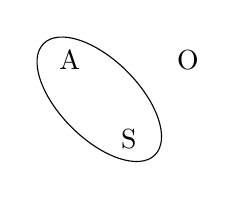
\begin{tikzpicture}
    \node[] at (0,1) {A};
    \node[] at (1.5,1) {O};
    \node[] at (0.75,0) {S};

    \draw[rotate around={45:(0.375,0.5)}] (0.375,0.5) ellipse (0.5 and 1);
  \end{tikzpicture}
  \caption{Nominative-accusative alignment}
  \label{fig:nom-acc-lang}
\end{figure}

In ergative-absolutive languages, the alignment is different. The subject of an intransitive verb (S) has the same marking as the object of the transitive verb (O), namely absolutive. The subject of the transitive verb (A) has its own marking, namely ergative. This is schematically shown in \ref{fig:erg-abs-lang}.

\begin{figure}[ht]
  \centering
  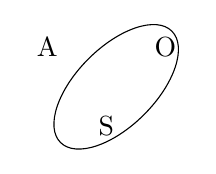
\begin{tikzpicture}
    \node[] at (0,1) {A};
    \node[] at (1.5,1) {O};
    \node[] at (0.75,0) {S};

    \draw[rotate around={135:(0.875,0.5)}] (0.875,0.5) ellipse (0.5 and 1);
  \end{tikzpicture}
  \caption{Ergative-absolutive alignment}
  \label{fig:erg-abs-lang}
\end{figure}

Note here that nominative-accusative languages use the same case marking for the same grammatical function (nominative for subject accusative for object), but ergative-absolutive languages do not.

\citet{bobaljik2006} describes how absolutives and ergatives behave with respect to whether they show agreement. There are languages in which there is agreement with both absolutives and ergatives. Besides that, there are languages in which there is only agreement with absolutives. Crucially, there is no language in which there is only agreement with ergatives. Absolutives are a heterogenous set with respect to grammatical function, i.e. they are subjects of intransitive verbs and objects of transitive verbs. However, with respect to showing agreement absolutives behave the same, and this behaviors is different from ergatives. This indicates that it is morphological case and not grammatical function that is the decisive factor.

\citeauthor{bobaljik2006} (following \citealt{marantz2000}) combines nominative-accusative and ergative-absolutive languages in the following way: accusative and ergative are dependent cases, and nominative or absolutive are unmarked case. Reformulating Figure \ref{fig:agr-sub-do-io} in terms of case instead of grammatical function gives the schema in Figure \ref{fig:agr-nom-acc-dat}.

\begin{figure}[H]
  \centering
  \begin{tikzpicture}
    \draw (0,1) circle (2.25);
    \draw [fill opacity=0.4, fill=LG] (0,0.5) circle (1.75);
    \draw [fill opacity=0.4, fill=DG] (0,0) circle (1.25);

    \node[] at (0,2.75) {unmarked case};
    \node[] at (0,1.5) {dependent case};
    \node[] at (0,0) {dative};

    \node[] at (2.5,3) {\footnotesize{● Japanese}};
    \node[] at (2.25,2) {\footnotesize{● German}};
    \node[] at (2,1) {\footnotesize{● Hungarian}};
    \node[] at (1.375,0) {\footnotesize{● Basque}};
  \end{tikzpicture}
  \caption{\posscitealt{bobaljik2006} actual schema}
  \label{fig:agr-def-dep-dat}
\end{figure}

This formulation in terms of case rather than grammatical function works as follows for the examples I gave earlier.
First, Japanese is a language that does not show any agreement, as shown in \ref{ex:japanese-agr}. There is no agreement with the unmarked case (here the nominative), not with the dependent case (here the accusative) and not with the dative case.
Second, German is a language that shows agreement only with the unmarked case, as shown in \ref{ex:german-agr}. The morpheme \tit{-st} on the predicate agrees with the element in unmarked nominative case \tit{du} `you'. There is no agreement with the dependent accusative case or with the dative case.
Third, Hungarian is a language that shows agreement with the unmarked and the dependent case, as shown in \ref{ex:hungarian-agr}. The portmanteau morpheme \tit{-om} on the predicates agrees with the element in unmarked nominative case \tit{én} `I' and the element in dependent accusative case \tit{a könyvet} `the book'.
Last, Basque is a language that shows agreement with the unmarked, the dependent and the dative case, as shown in \ref{ex:basque-agr}. The morpheme \tit{-zu} on the auxiliary agrees with the element in dependent ergative case \tit{zuk} `you'. The morpheme \tit{d-} on the auxiliary agrees with the element in unmarked absolutive case \tit{liburua} `the book'. The morpheme \tit{-ta} on the auxiliary agrees with the element in dative case \tit{niri} `me'.

In the languages I discuss in this dissertation, I focus on languages that have nominative as unmarked case and accusative as dependent case, so Figure \ref{fig:agr-nom-acc-dat} suffices.

\begin{figure}[ht]
  \centering
  \begin{tikzpicture}
    \draw (0,1) circle (2.25);
    \draw [fill opacity=0.4, fill=LG] (0,0.5) circle (1.75);
    \draw [fill opacity=0.4, fill=DG] (0,0) circle (1.25);

    \node[] at (0,2.75) {\ac{nom}};
    \node[] at (0,1.75) {\ac{acc}};
    \node[] at (0,0) {\ac{dat}};
  \end{tikzpicture}
  \label{fig:agr-nom-acc-dat}
  \caption{\posscitealt{bobaljik2006} simplified schema}
\end{figure}

In sum, this section has shown that agreement follows the same implicational hierarchy as the case scale in headless relatives: \ac{nom} < \ac{acc} < \ac{dat}.


\subsection{Relativization}

Relativization refers to the process in which a relative clause is derived from a non-relative clause. An example of the non-relative clause is given in \ref{ex:rel-non}. The relative clause derived from that is shown in \ref{ex:rel-realati}. The head of the relative clause is \tit{woman} and precedes the clause. The relative pronoun follows the head. The head of the head does not appear in the relative clause anymore.

\ex.
\a. You like the woman. \label{ex:rel-non}
\b. \tbf{the} \tbf{woman}, who you like \label{ex:rel-realati}

In \ref{ex:rel-realati}, it is the object of the clause that is relativized. It differs per language which elements can be relativized with a particular strategy. Just like the distribution was not random for agreement, it is not random which elements can be relativized. Instead, there is an implicational hierarchy that is identical to the one observed for the case scale: \ac{nom} < \ac{acc} < \ac{dat}.

\citet{keenan1977} formulated the implicational hierarchy in terms of the grammatical functions subject, direct object and indirect object.\footnote{
\citet{keenan1977} also included obliques, possessives and objects of comparison on the lowest end of the hierarchy. I leave them out here, because they are not relevant for the discussion.
}
The implicational hierarchy is schematically represented in Figure \ref{fig:rel-sub-do-io}. It should be read as follows: if a language allows a particular relativization strategy of the grammatical function in a particular circle, it also allows this relativization strategy of the grammatical function of the circle around it. The languages in the figure give examples of the circles they are in.

\begin{figure}[ht]
  \centering
  \begin{tikzpicture}
    \draw (0,1) circle (2.25);
    \draw [fill opacity=0.4, fill=LG] (0,0.5) circle (1.75);
    \draw [fill opacity=0.4, fill=DG] (0,0) circle (1.25);

    \node[] at (0,2.75) {subject};
    \node[] at (0,1.5) {direct object};
    \node[align=center] at (0,0) {indirect\\ object};

    \node[] at (2.25,2) {\footnotesize{● Malagasy/German}};
    \node[] at (2,1) {\footnotesize{● Malay}};
    \node[] at (1.375,0) {\footnotesize{● Basque}};
  \end{tikzpicture}
  \caption{Schema for relativization}
  \label{fig:rel-sub-do-io}
\end{figure}

There are four types of languages possible: first, a language that allows only the subject to be relativized with a particular strategy and not the direct and indirect object; second, a language that allows the subject and direct object to be relativized with a particular strategy but not the indirect object; and third, a language that allows the subject, the direct object and the indirect object to be relativized with a particular strategy.

Malagasy is an example of a language that allows subjects to be relativized using a particular strategy, but not direct and indirect objects. \ref{ex:malagasy-decl} is an example of a declarative sentence in Malagasy. It is a transitive sentence that contains the subject \tit{ny mpianatra} `the student' and the direct object \tit{ny vehivavy} `the woman'.

\exg. Nahita ny vehivavy ny mpianatra.\\
 saw the woman the student\\
 `The student saw the woman.' \flushfill{Malagasy, \pgcitealt{keenan1977}{70}}\label{ex:malagasy-decl}

In \ref{ex:malagasy-subj}, the subject from the declarative sentence, marked in bold, is relativized. The subject \tit{ny mpianatra} `the student' appears in the first position of the clause. It is followed by the invariable relativizer \tit{izay} `that'. After that, the rest of the relative clause follows, in this case \tit{nahita ny vehivavy} `saw the woman'.

\exg. \tbf{ny} \tbf{mpianatra} izay nahita ny vehivavy\\
 the student that saw the woman\\
 `the student that saw the woman' \flushfill{Malagasy, \pgcitealt{keenan1977}{70}, my boldfacing}\label{ex:malagasy-subj}

The object of \ref{ex:malagasy-decl} cannot be relativized in the same way, as shown in \ref{ex:malagasy-no-do}. Here the object \tit{ny vehivavy} `the woman', marked in bold, appears in the first position of the clause. It is again followed by the relativizer \tit{izay} `that' and the rest of the relative clause, which is here \tit{nahita ny mpianatra} `saw the student'. This example is ungrammatical.

\exg. *\tbf{ny} \tbf{vehivavy} izay nahita ny mpianatra\\
 the woman that saw the student\\
 `the woman that the student saw' \flushfill{Malagasy, \pgcitealt{keenan1977}{70}, my boldfacing}\label{ex:malagasy-no-do}

Later in this section I draw the parallel between subject and nominative, direct object and accusative and indirect object and dative \citep[after][]{caha2009}. As Malagasy does not have any overt morphological system, it does not hold that the subject corresponds to the nominative in this case.
German is another example of a language that allows subjects to be relativized using a particular strategy, but not direct and indirect object. This strategy is the participle construction \citep{keenan1977}. This strategy is a secondary strategy that exist besides the main strategy that can be used to relativize direct and indirect objects. \ref{ex:german-rel-decl} is an example of a declarative sentence in German. It is a transitive sentence that contains the subject \tit{die Frau} `the woman' and the object \tit{der Mann} `the man'.

\exg. Die Frau küsst den Mann.\\
the woman kisses the man\\
`The woman is kissing the man.' \flushfill{German}\label{ex:german-rel-decl}

The subject from the declarative in \ref{ex:german-rel-decl}, sentence \tit{die Frau} `the woman', is relativized in \ref{ex:german-rel-subj}. The predicate from the declarative clause \tit{küsst} `kisses' is turned in into the participle \tit{küssende} `kissing'. The participle appears at the end of the reduced relative clause \tit{den Mann küssende} `the man kissing'. The reduced relative clause directly precedes the noun of the subject, creating distance between the determiner \tit{die} `the' and \tit{Frau} `woman', which are both marked in bold.

\exg. \tbf{die} den Mann küssende \tbf{Frau}\\
 the the man kissing woman\\
 `the woman who is kissing the man' \flushfill{German}\label{ex:german-rel-subj}

The object from the declarative sentence in \ref{ex:german-rel-decl}, \tit{den Mann} `the man', cannot be relativized like the subject, as shown in \ref{ex:german-rel-no-do}. Again, the predicate from the declarative clause \tit{küsst} `kisses' is turned in into the participle \tit{küssende} `kissing'. The participle appears at the end of the relative clause \tit{die Frau küssende} `the woman kissing'. The reduced relative clause directly precedes the noun of the object, creating distance between the determiner \tit{der} `the' and \tit{Mann} `man', which are both marked in bold. This example is ungrammatical.

\exg. *\tbf{den} die Frau küssende \tbf{Mann}\\
 the the woman kissing man\\
 intended: `the man that the woman is kissing' \flushfill{German}\label{ex:german-rel-no-do}

Malay is an example of a language that has a relativization strategy for subjects and direct objects, but not for indirect objects. \ref{ex:malay-do} shows an example in which the object is relativized. The object here is \tit{ayam} `chicken', marked in bold. It is followed by the relativizer \tit{yang} `that'. After that, the rest of the relative clause \tit{Aminah sedang memakan} `Aminah is eating' follows. The same strategy works to relativize subjects, which is not illustrated with an example.

\exg. Ali bunoh \tbf{ayam} yang Aminah sedang memakan.\\
 Ali kill chicken that Aminah \ac{prog} eat\\
 `Ali killed the chicken that Aminah is eating.' \flushfill{Malay, \pgcitealt{keenan1977}{71}, my boldfacing}\label{ex:malay-do}

Indirect objects cannot be relativized using the same strategy. \ref{ex:malay-decl} is an example of a ditransitive sentence in Malay. The indirect object \tit{kapada perempuan itu} `to the woman' cannot be relativized using \tit{yang}.

\exg. Ali beri {ubi kentang} itu kapada perempuan itu.\\
 Ali give potato the to woman the\\
 `Ali gave the potato to the woman.'\label{ex:malay-decl} \flushfill{Malay, \pgcitealt{keenan1977}{71}}

This is illustrated by the examples in \ref{ex:malay-no-io}. In \ref{ex:malay-no-io1}, the direct object \tit{perempuan kapada} `to the woman', marked in bold, appears in the first position of the clause. It is followed by the relativizer \tit{yang} `that' and the rest of the relative clause \tit{Ali beri ubi kentang itu kapada} `Ali gave the potato to'. This example in ungrammatical.
The example in \ref{ex:malay-no-io2} differs from \ref{ex:malay-no-io1} in that the preposition \tit{kapada} `to' has been moved such that it precedes the relativizer \tit{yang} `that'. This example is ungrammatical as well, indicating this was not the reason for the ungrammaticality.

\ex.\label{ex:malay-no-io}
\ag. *\tbf{perempuan} yang Ali beri {ubi kentang} itu kapada\\
 woman that Ali give potato the to\\\label{ex:malay-no-io1}
\bg. *\tbf{perempuan} \tbf{kapada} yang Ali beri {ubi kentang} itu\\
 woman to who Ali give potato that\\\flushfill{Malay, \pgcitealt{keenan1977}{71}, my boldfacing}\label{ex:malay-no-io2}

% Later in this section I draw the parallel between subject and nominative, direct object and accusative and indirect object and dative \citep[after][]{caha2009}. As Malagasy does not have any overt morphological system, it does not hold that the subject corresponds to the nominative in this case.
% Finnish is another example..
%
%  (12) a. Poydalla tanssinut poika oli sairas.
%  on-table having-danced boy was sick
%  'The boy who had danced on the table was sick.'
%  b. Nakemani poika tanssi poydalla.
%  I-having-seen boy danced on-table
%  'The boy that I saw danced on the table.'



Basque is an example of a language that has a particular relativization strategy for subjects, direct objects and indirect objects. \ref{ex:basque-decl} is an example of a declarative ditransitive sentence in Basque. The sentence contains the subject \tit{gizonak} `the man', the direct object \tit{liburua} `the book' and the indirect object \tit{emakumeari} `the woman'.

\exg. Gizon-a-k emakume-a-ri liburu-a eman dio.\\
 man-\ac{def}-\ac{erg} woman-\ac{def}-\ac{dat} book-\ac{def}.\ac{abs} give has\\
 `The man has given the book to the woman.' \flushfill{Basque, \pgcitealt{keenan1977}{72}}\label{ex:basque-decl}

A relative clause in Basque appears in the prenominal position and it is marked by the invariable marker \tit{-n}.\footnote{
Additionally, the relativized positions do not appear in verbal agreement anymore, but this not visible in the example, because they are all phonologically zero.
}
\ref{ex:basque-sub} shows the three relativizations that are derived from \ref{ex:basque-decl}.
In \ref{ex:basque-sub}, the ergative subject \tit{gizonak} `the man' from \ref{ex:basque-decl} is relativized. The head \tit{gizona} `the man', marked in bold, has lost its ergative marker \tit{-k}, and follows the relative clause \tit{makumeari liburua eman dio} `who has given the book to the woman'. The suffix \tit{-n} is attached to the relative clause.
In \ref{ex:basque-do}, the absolutive direct object \tit{liburua} `the book' from \ref{ex:basque-decl} is relativized. The head \tit{liburua} `the book', marked in bold, follows the relative clause \tit{gizonak emakumeari eman dion} `that the man has given to the woman'.\footnote{
The absolutive direct object \tit{liburua} `the book' does not have an additional overt absolutive marker, so this difference cannot be observed when it is relativized.
}
The suffix \tit{-n} is attached to the relative clause.
In \ref{ex:basque-io}, the dative indirect object \tit{emakumeari} `the woman' from \ref{ex:basque-decl} is relativized. The head \tit{emakumea} `the man', marked in bold, has lost its dative marker \tit{-ri}, and follows the relative clause \tit{gizonak liburua eman dion} `that the man has given the book to'. The suffix \tit{-n} is attached to the relative clause.

\ex.\label{ex:basque-rel}
\ag. emakume-a-ri liburu-a eman dio-n \tbf{gizon-a}\\
 woman-\ac{def}-\ac{dat} book-\ac{def}.\ac{abs} give has-\ac{rel} man-\ac{def}\\
 `the man who has given the book to the woman'\label{ex:basque-sub}
\bg. gizon-a-k emakume-a-ri eman dio-n \tbf{liburu-a}\\
 man-\ac{def}-\ac{erg} woman-\ac{def}-\ac{dat} give has-\ac{rel} book-\ac{def}\\
 `the book that the man has given to the woman'\label{ex:basque-do}
\bg. gizon-a-k liburu-a eman dio-n \tbf{emakume-a}\\
 man-\ac{def}-\ac{erg} book-\ac{def}.\ac{abs} give has-\ac{rel} woman-\ac{def}\\
 `the woman that the man has given the book to' \flushfill{Basque, \pgcitealt{keenan1977}{72}, my boldfacing}\label{ex:basque-io}

\citet{caha2009} argues that the implicational hierarchy is more accurate if it is stated in terms of case rather than grammatical function. The main argument comes from ergative-absolutive languages, which was also one of \posscitet{bobaljik2006} argument with the implicational hierarchy for agreement. \citet{keenan1977} point out that some ergative-absolutive languages form a counterexample to their hierarchy. \citet{caha2009} points out that ergative subjects and oblique noun phrases use the same relativization strategy, which is not allowed with absolutive objects (which is also briefly mentioned in
\citealt{bobaljik2006}).

Reformulating Figure \ref{fig:agr-sub-do-io} in terms of case instead of grammatical function gives the schema in Figure \ref{fig:agr-nom-acc-dat}.

\begin{figure}[ht]
  \centering
  \begin{tikzpicture}
    \draw (0,1) circle (2.25);
    \draw [fill opacity=0.4, fill=LG] (0,0.5) circle (1.75);
    \draw [fill opacity=0.4, fill=DG] (0,0) circle (1.25);

    \node[] at (0,2.75) {unmarked case};
    \node[] at (0,1.5) {dependent case};
    \node[align=center] at (0,0) {dative};

    \node[] at (2.25,2) {\footnotesize{● Malagasy/German}};
    \node[] at (2,1) {\footnotesize{● Malay}};
    \node[] at (1.375,0) {\footnotesize{● Basque}};
  \end{tikzpicture}
  \caption{Schema for relativization}
  \label{fig:rel-def-dep-dat}
\end{figure}

This formulation in terms of case rather than grammatical function works as follows for the examples I gave earlier.

First, German is a language that has a particular relativization strategy for the unmarked case, as shown in \ref{ex:german-rel-subj}. The unmarked nominative case can be relativized with a reduced relative clause, but the dependent accusative case and the dative case cannot.
Second,
Last, Basque is a language that has a particular relativization strategy for unmarked, dependent and dative case, as shown in \ref{ex:basque-rel}. The unmarked ergative, dependent absolutive and dative case can be relativized by extraposing the head, and marking it with the invariable marker \tit{-n}.

In the languages I discuss in this dissertation, I focus on languages that have nominative as unmarked case and accusative as dependent case, so Figure \ref{fig:rel-nom-acc-dat} suffices.

\begin{figure}[ht]
  \centering
  \begin{tikzpicture}
    \draw (0,1) circle (2.25);
    \draw [fill opacity=0.4, fill=LG] (0,0.5) circle (1.75);
    \draw [fill opacity=0.4, fill=DG] (0,0) circle (1.25);

    \node[] at (0,2.75) {nominative};
    \node[] at (0,1.5) {accusative};
    \node[align=center] at (0,0) {dative};
  \end{tikzpicture}
  \caption{Schema for relativization}
  \label{fig:rel-nom-acc-dat}
\end{figure}

In sum, this section has shown that relativization follows the same implicational hierarchy as agreement and as the case scale in headless relatives: \ac{nom} < \ac{acc} < \ac{dat}.


\section{In morphology}\label{sec:case-morphology}

In the two previous sections I showed that the case scale \ac{nom} < \ac{acc} < \ac{dat} can be observed in three syntactic phenomena. First, it shows up in case competition in headless relatives. Second, the case scale forms the basis for the implicational hierarchy observed in agreement across languages. Third, the identical implicational holds for relativization strategies cross-linguistically.

In this section, I show that this same case scale also shows up in morphology. First, syncretism only targets continuous regions on the case scale. Second, several languages show formal containment that mirrors the case scale.


\subsection{Syncretism}

Syncretism refers to the phenomenon whereby two or more different functions are fulfilled by a single form \citep[cf.][]{baerman2002}. In this section I discuss literature that shows that syncretism patterns among nominative, accusative and dative are not random. Instead, they pattern along the case scale \ac{nom} < \ac{acc} < \ac{dat}.

It has widely been observed that syncretism is restricted by the linear sequence \ac{nom} --- \ac{acc} --- \ac{dat} \citep{baerman2005,caha2009,zompi2017} (and see \citealt{mcfadden2018,smith2019} for similar claims concerning root suppletion). That is, if one orders cases in this linear sequence, only contiguous regions in the sequence turn out to be syncretic.
Following that, four possible patterns are attested crosslinguistically. First, all three cases are syncretic. Second, nominative and accusative are syncretic and the dative is not. Third, the accusative and the dative are syncretic and the nominative is not. Fourth, all cases are non-syncretic.

There is one pattern that is not attested crosslinguistically. This pattern does not target continuous regions, but non-contiguous ones: nominative and dative are syncretic and accusative is not. In other words, there is no ABA pattern (in which a form B intervenes between the two identically formed As) \citep{bobaljik2012}.

Table \ref{tbl:syncretisms} shows examples for each of these possible patterns.
I give an example from three distinct forms from Faroese. The second person singular is \tit{tú} `you' for nominative, \tit{teg} `you' for accusative and \tit{tær} `you' for dative \pgcitep{lockwood1977}{70}.
I give an example from a syncretism between nominative, accusative and dative from Dutch. The second person plural pronoun is \tit{jullie} `you.\ac{pl}' is syncretic between nominative, accusative and dative.
I give an example from a syncretism between accusative and dative but not nominative from Icelandic. The first person singular plural is \tit{okkur} `us' is syncretic between accusative and dative. The nominative has a separate form: \tit{við} `we' \pgcitep{einarsson1949}{68}.
I give an example from a syncretism between nominative and accusative but not dative from German. The third person singular feminine \tit{sie} `she/her' is syncretic between nominative and accusative. The dative has a separate form: \tit{ihr} `her'.
Crucially, to the best of my knowledge, there is no language in which the nominative and the dative are syncretic but the accusative is not.

\begin{table}[ht]
  \center
  \caption {}
    % !TEX root = ../thesis.tex

\begin{tabular}{cccccccc}
  \toprule
      \multicolumn{3}{c}{pattern}
        & \ac{nom}
        & \ac{acc}
        & \ac{dat}
        & translation
        & language \\
  \cmidrule(lr){1-3} \cmidrule(lr){4-6} \cmidrule(lr){7-7} \cmidrule(lr){8-8}
      A & A & A
        & \cellcolor{LG}jullie
        & \cellcolor{LG}jullie
        & \cellcolor{LG}jullie
        & 2\ac{pl}
        & Dutch \\
      A & A & B
        & \cellcolor{LG}sie
        & \cellcolor{LG}sie
        & ihr
        & 3\ac{sg}.\ac{f}
        & German \\
      A & B & B
        & við
        & \cellcolor{LG}okkur
        & \cellcolor{LG}okkur
        & 1\ac{pl}
        & Icelandic \\
      A & B & C
        & tú
        & teg
        & tær
        & 2\ac{sg}
        & Faroese \\
      A & B & A
        & \cellcolor{LG}
        &
        & \cellcolor{LG}
        &
        & not attested \\
  \bottomrule
\end{tabular}

  \label{tbl:syncretisms}
\end{table}

In sum, case syncretism follows the ordering of the case scale in headless relatives: \ac{nom} < \ac{acc} < \ac{dat}.


\subsection{Formal containment}

This section shows a second way in which \ac{nom} < \ac{acc} < \ac{dat} is reflected in morphology: formal containment \citep[cf.][]{smith2019,zompi2017,caha2010}. In some languages, the form that is used for the accusative literally contains the form that is used for the nominative. In turn, the forms for the dative contains the form for the accusative. I illustrate this phenomenon with examples from Khanty.

Khanty (or Ostyak) shows formal containment in some of its pronouns (\pgcitealt{nikolaeva1999}{16} after \citealt{smith2019}). Three examples are given in Table \ref{tbl:cont-khanty}.

The nominative form for the first person singular is \tit{ma} `I.\ac{nom}'. The form for the accusative is \tit{ma:ne:m} `me'. This is the form for the nominative \tit{ma} plus the accusative marker \tit{-ne:m}. The form for the dative is \tit{ma:ne:mna} `me'. This is the form for the accusative \tit{ma:ne:m} plus the dative marker \tit{-na}. So, dative formally contains the accusative, and the accusative formally contains the nominative.

The third person singular and first person plural show the same pattern. The accusative forms \tit{luwe:l} `him/her' and \tit{muŋe:w} `us' contain the nominative forms \tit{luw} and the \tit{muŋ} plus the accusative marker \tit{-e:l} or \tit{-e:w}. The dative forms \tit{luwe:lna} `him/her' and \tit{muŋe:wna} `us' contain the accusative forms \tit{luwe:l} and \tit{muŋe:w} plus the dative marker \tit{-na}. Again, the dative formally contains the accusative, which in turn contains the nominative.

\begin{table}[ht]
  \center
  \caption {Case containment in Khanty}
  \begin{tabular}{clll}
  \toprule
            & \ac{1}\ac{sg}
            & \ac{3}\ac{sg}
            & \ac{1}\ac{pl}                           \\
            \cmidrule{2-4}
  \ac{nom}  & ma
            & luw
            & muŋ                                     \\
  \ac{acc}  & ma:\tbf{-ne:m}
            & luw\tbf{-e:l}
            & muŋ\tbf{-e:w}                           \\
  \ac{dat}  & ma:\tbf{-ne:m}\tcol{DG}{\tbf{-na}}
            & luw\tbf{-e:l}\tcol{DG}{\tbf{-na}}
            & muŋ\tbf{-e:w}\tcol{DG}{\tbf{-na}}       \\
  \bottomrule
  \end{tabular}
  \label{tbl:cont-khanty}
\end{table}

Other languages that show this phenomenon are West Tocharian \citep{gippert1987} and Vlakh and Kalderaš Romani (respectively \citealt{friedman1991} and \citealt{boretzky1994}).

In sum, some languages morphologically look like \ac{nom}-\ac{acc}-\ac{dat}. This exactly reflects the case scale \ac{nom} < \ac{acc} < \ac{dat}.

\section{Summary}

Case competition in headless relatives adheres to the case scale in \ref{ex:case-scale-sum}. If the internal and external case differ, cases more on the right of the scale win over cases more to the left on the case.

\ex. \ac{nom} < \ac{acc} < \ac{dat}\label{ex:case-scale-sum}

This case scale is not only found in case competition in headless relatives. Implicational hierarchies regarding two syntactic phenomena appear across languages. The first one concerns agreement. If a language shows agreement with datives, it also shows agreement with accusatives and nominatives. If a language shows agreement with accusatives, it also shows agreement with nominatives.
The second implicational hierarchy concerns relativization. If a dative in a language can be relativized with a particular strategy, an accusative and a nominative can be too using the same strategy. If an accusative can be relativized with a particular strategy, so can a nominative with this strategy.

The case scale also shows up in morphological patterns. First, if the cases are ordered according to the case scale, syncretism only target continuous forms, no ABA pattern appears. Second, some languages show how the dative formally contains accusative, and how the accusative formally contains the nominative.

These phenomena show that the pattern observed in headless relatives is not something that stands on itself. The scale is a pattern that recurs across languages and across different phenomena. Therefore, it should not be treated as an special process with its own stipulated rule. Instead, it is something general that should also follow from general processes in languages.

The next chapter shows how features of the nominative, accusative and dative are organized. All facts presented in this chapter can be derived from the organization of these features.

% !TEX root = thesis.tex

\chapter{Case decomposition}\label{ch:decomposition}

This chapter provides a theory that derives the first aspect of case competition in headless relatives that I discuss in this dissertation.
This theory seeks to capture that headless relatives crosslinguistically adhere to the case scale \tsc{nom} < \tsc{acc} < \tsc{dat}.

In most existing accounts for case competition in headless relatives (\citealt[cf.][]{pittner1995,vogel2001,grosu2003,harbert1978}, an exception to this is \citealt{himmelreich2017}) the case scale is stipulated. Headless relatives are said to simply obey to that scale. \pgcitet{pittner1995}{fn.4} makes this explicit: ``One of the reviewers notes that an explanation in terms of a Case hierarchy is rather stipulative. However, as far as I know, nobody has suggested a nonstipulative explanation for these facts.''

In the previous chapter I showed that the case scale \ac{nom} < \ac{acc} < \ac{dat} is not specific to headless relatives, but it is a wide-spread phenomenon: it can also be observed in morphology (and in syntax).

Within morphology it appears in syncretism patterns and morphological case containment. \pgcitet{pittner1995}{201:fn.4} makes this link to morphology as well: ``Furthermore, the Case hierarchies receive some independent support by morphology as shown by the various inflectional paradigms.''

As I already eluded to in the summary of Chapter \ref{ch:introduction}, I am not after a theory in which the case scale is something construction-specific, or one in which syntax and morphology both have their own case scale. Instead, argue that there is a single trigger that is responsible for the case scales in different subparts of language (which is identical to what \citealt{caha2019} suggests for case competition in numeral phrases). Specifically, I show that the observed case scale naturally follows on the assumption that the case scale is deeply anchored in syntax. The case scales in morphology and syntax are merely reflexes of how case is organized in the linguistic system.\footnote{
\citet{himmelreich2017} works this intuition out in a different way.
}

This chapter is structured as follows. First, I introduce a specific cumulative case decomposition \citep{caha2009}. In the two following sections, I show how this case decomposition is able to derive the syncretism and morphological case containment facts from Chapter \ref{ch:recurring}. I make this concrete in the framework Nanosyntax \citep{starke2009}. Finally, I show how the case decomposition relates to the winner in case competition in headless relatives.


\section{The basic idea}

\citet{caha2009,caha2013} (followed by \citealt[cf.][]{starke2009,bobaljik2012,mcfadden2018,smith2019,vanbaal2018}) has extensively argued that case should be decomposed into privative features. Specifically, the decomposition is cumulative: each case has a different number of case features, and the number grows one by one.
This is illustrated in Table \ref{tbl:case-decomposed}. Accusative has all the features that nominative has (here \tsc{k}1) plus one extra (here \tsc{k}2). Dative has all the features accusative has (\tsc{k}1 and \tsc{k}2) plus one extra (\tsc{k}3).

\begin{table}[ht]
  \center
	\caption {Cumulative case decomposition}
		\begin{tabular}{ll}
    \toprule
    case      & features                  \\
    \midrule
    \ac{nom} & \tsc{k}1                    \\
    \ac{acc} & \tsc{k}1, \tsc{k}2           \\
    \ac{dat} & \tsc{k}1, \tsc{k}2, \tsc{k}3  \\
    \bottomrule
    \end{tabular}
    \label{tbl:case-decomposed}
\end{table}

Consider the case scale, repeated in repeated in \ref{ex:case-scale-derive}.

\ex. \ac{nom} < \ac{acc} < \ac{dat}\label{ex:case-scale-derive}

This scale actually indicates containment.
Nominative corresponds to a set of features (\tsc{k}1) that is contained in the set of features of accusative (\tsc{k}1 and \tsc{k}2).
Similarly, nominative corresponds to a set of features that is contained in the set of features of dative (\tsc{k}1, \tsc{k}2 and \tsc{k}3).
Lastly, accusative corresponds to a set of features (\tsc{k}1 and \tsc{k}2) that is contained in the set of features of dative (\tsc{k}1, \tsc{k}2 and \tsc{k}3).

The decomposition in Table \ref{tbl:case-decomposed} forms the basis to derive the case scale effects observed in Chapter \ref{ch:recurring}. The following sections show how morphological case containment and syncretism effects follow naturally. After that, I show how the decomposition also derives the case competition facts in headless relatives.


\section{Deriving syncretism}\label{sec:syncretism}

Case syncretism follows the ordering of the case scale. Along this scale, only contiguous regions in the sequence are syncretic. In this section I show how case syncretism patterns can be derived from the case decomposition shown in Table \ref{tbl:case-decomposed}.
In Table \ref{tbl:syncretisms-derive} I repeat the examples that shows the possible and impossible syncretism patterns.

\begin{table}[ht]
  \center
  \caption {Syncretism patterns in Germanic pronouns (repeated)}
    % !TEX root = ../thesis.tex

\begin{tabular}{cccccccc}
  \toprule
      \multicolumn{3}{c}{pattern}
        & \ac{nom}
        & \ac{acc}
        & \ac{dat}
        & translation
        & language \\
  \cmidrule(lr){1-3} \cmidrule(lr){4-6} \cmidrule(lr){7-7} \cmidrule(lr){8-8}
      A & A & A
        & \cellcolor{LG}jullie
        & \cellcolor{LG}jullie
        & \cellcolor{LG}jullie
        & 2\ac{pl}
        & Dutch \\
      A & A & B
        & \cellcolor{LG}sie
        & \cellcolor{LG}sie
        & ihr
        & 3\ac{sg}.\ac{f}
        & German \\
      A & B & B
        & við
        & \cellcolor{LG}okkur
        & \cellcolor{LG}okkur
        & 1\ac{pl}
        & Icelandic \\
      A & B & C
        & tú
        & teg
        & tær
        & 2\ac{sg}
        & Faroese \\
      A & B & A
        & \cellcolor{LG}
        &
        & \cellcolor{LG}
        &
        & not attested \\
  \bottomrule
\end{tabular}

  \label{tbl:syncretisms-derive}
\end{table}

Table \ref{tbl:syncretisms-derive} shows that if one orders cases in the linear sequence \ac{nom} --- \ac{acc} --- \ac{dat}, only contiguous regions in the sequence turn out to be syncretic. First, all three cases can be non-syncretic, as in Faroese. Second, all three cases can be syncretic, as in Dutch. Third, the accusative and the dative can be syncretic and the nominative not, as in Icelandic. Fourth, nominative and accusative can be syncretic and the dative not, as in German. The pattern that is not attested crosslinguistically is the one that targets non-contiguous regions in the table, the ABA pattern \citep{baerman2005,caha2009,zompi2017}.

The syncretism facts follow in a system in which the case is decomposed as in Table \ref{tbl:case-decomposed} and in which lexicalization relies on containment. The latter means that a phonological form is not only inserted when the lexical specification is identical to the syntax, but also when the syntactic features are a subset of the lexical specification. The intuition is the following. Syncretic forms are realized by a single `lexical entry' from the `lexicon'. I elaborate on the terms lexical entry and lexicon shortly.
A lexical entry can be applied if it contains all features, as long as there is no more specific one. This system can generate the patterns ABC, AAA, ABB and AAB, but not ABA.

Before I show how the four attested patterns can be derived (and the unattested one cannot), I need to make some theoretical assumptions explicit about Nanosyntax, the framework in which this dissertation is worked out. First, I show how the Nanosyntactic system is set up in such a way that morphological patterns (like syncretism, but also morphological containment) can inform us about the way syntax is structured. Therefore, I briefly discuss the general architecture of Nanosyntax, its postsyntactic lexicon, and the content and shape of lexical entries. Lastly, I discuss how multiple features (like \tsc{k}1, \tsc{k}2 and \tsc{k}3 from Table \ref{tbl:case-decomposed}) can be spelled out by a single phonological element using phrasal spellout.

In Nanosyntax, syntax starts with atomic features, and it builds complex syntactic trees. Specifically, there are no `feature bundles' (from a pre-syntactic lexicon) that enter the syntax. The only way complex feature structures come to exist is a a result of merge.
After syntax (actually, each instance of merge), the syntactic structure is matched against the lexicon for pronunciation. The lexicon `translates' between lexical trees (i.e. syntactic representations) on the one hand and phonology (PF) and concepts (CF) on the other hand.\footnote{
Throughout the dissertation I call the syntactic representations in the lexicon `lexical trees' in order to distinguish them from syntactic structures in the syntax.
}

In Nanosyntax, the lexicon contains lexical entries, which are links between lexical trees, phonological representations and conceptual representations \citep{starke2014}.\footnote{
The lexical tree does not have to correspond to both a phonological and a conceptual representation. Lexical trees that only correspond to a conceptual representations and not to phonological representations are (phrasal or clausal) idioms. Lexical trees that only correspond to phonological representations but not to conceptual representations are for instance irregular plurals.
} I leave the conceptual representation out of discussion for now, as it is not relevant for the discussion here. The fact that only syntax can create complex feature structures also has a consequence for lexical entries in the lexicon.
Syntactic structures are constrained by certain principles, such that only well-formed syntactic structures exist. Since lexical entries in the lexicon link lexical trees to phonological and conceptual representation, these lexical trees are constrained by the same principles as syntactic structures are.
As a result, the lexicon only contains well-formed lexical trees. The lexicon does not contain unstructured `feature bundles', because they could never be created by syntax.

Following this logic, a feature bundle as in \ref{ex:feature-set} cannot exist. It cannot have entered syntax, because syntax starts with atomic features. It can also not be created by syntax, because complex structures can only be created with merge.

\ex. [ \tsc{k}1, \tsc{k}2, \tsc{k}3 ]\label{ex:feature-set}

Instead, a possible lexical tree looks as in \ref{ex:feature-structure}. The features are merged one by one in a binary structure.

\ex. \begin{forest} boom
  [\ac{dat}P
      [\tsc{k}3]
      [\ac{acc}P
          [\tsc{k}2]
          [\tsc{k}1]
      ]
  ]
\end{forest}\label{ex:feature-structure}

This structure leads to the concept of phrasal spellout: not terminals but multiple syntactic heads (phrases) are realized with a single piece of phonology (i.e. a single morpheme). Applying this to \ref{ex:feature-structure}, not the terminals \tsc{k}1, \tsc{k}2 and \tsc{k}3 receive a realization, but \ac{acc}P and \ac{dat}P are spelled out. A necessary requirement is that these multiple syntactic heads form a constituent. That means that \ac{dat}P cannot be spelled out without \ac{acc}P.

Let me illustrate all of the above with the Faroese pronouns from Table \ref{tbl:syncretisms-derive}. I simplify the situation in two respects. First, I do not show the internal complexity of the pronouns, including person and number features. Instead, I give a triangle, indicating that this is a complex syntactic structure. I refer to is as the person-number phrase it refers to, e.g. 2\ac{sg}P. Second, in this simplified representation I consider the Faroese pronouns to be monomorphemic. I ignore the fact that all three pronouns have the stem \tit{t} with a suffix following it.

The lexical entry for \tit{tú} is given in \ref{ex:faroese-tu-lexicon}. The lexical tree consists of the second person singular pronoun (the 2\ac{sg}P), and \tsc{k}1, making it a \ac{nom}P. The phonological representation that is linked to the lexical tree is \tit{tú}.\footnote{
Throughout the dissertation, I use lexical trees and phonological forms connected by a double arrow (⇔) to refer to a lexical entry.
}

\ex.
\begin{forest} boom
  [\ac{nom}P
      [\tsc{k}1]
      [2\ac{sg}P
          [\phantom{xxx}, roof]
      ]
  ]
  {\draw (.east) node[right]{⇔ \tit{tú}}; }
\end{forest}
\label{ex:faroese-tu-lexicon}

The lexical entry for \tit{teg} is given in \ref{ex:faroese-teg-lexicon}. The lexical tree consists of all the features of the lexical tree in \ref{ex:faroese-tu-lexicon}, plus \tsc{k}2, making it an \ac{acc}P. The linked phonological representation is \tit{teg}.

\ex.
\begin{forest} boom
  [\ac{acc}P
      [\tsc{k}2]
      [\ac{nom}P
          [\tsc{k}1]
          [2\ac{sg}P
              [\phantom{xxx}, roof]
          ]
      ]
  ]
  {\draw (.east) node[right]{⇔ \tit{teg}}; }
\end{forest}
\label{ex:faroese-teg-lexicon}

The lexical entry for \tit{tær} is given in \ref{ex:faroese-taer-lexicon}. The lexical tree consists of all the features of the lexical tree in \ref{ex:faroese-teg-lexicon}, plus \tsc{k}3, making it an \ac{dat}P. The linked phonological representation is \tit{tær}.

\ex.
\begin{forest} boom
  [\ac{dat}P
      [\tsc{k}3]
      [\ac{acc}P
          [\tsc{k}2]
          [\ac{nom}P
              [\tsc{k}1]
              [2\ac{sg}P
                  [\phantom{xxx}, roof]
              ]
          ]
      ]
  ]
  {\draw (.east) node[right]{⇔ \tit{tær}}; }
\end{forest}
\label{ex:faroese-taer-lexicon}

The lexical trees and their phonological counterparts I gave in \ref{ex:faroese-tu-lexicon} to \ref{ex:faroese-taer-lexicon} are lexical entries.
These lexical entries are used to spell out syntactic structures. I give examples of syntactic structures in \ref{ex:faroese-tu-spellout} to \ref{ex:faroese-taer-spellout}.

The lexical tree in \ref{ex:faroese-tu-lexicon} is identical to the syntactic structure in \ref{ex:faroese-tu-spellout}. Therefore, this syntactic structure is spelled out as \tit{tú}.\footnote{
Throughout this dissertation I circle the part of the syntactic structure that corresponds to a particular lexical entry, and I place the corresponding phonology under it.
}

\ex. \begin{forest} boom
[\ac{nom}P,
tikz={
\node[label=below:\tit{tú},
draw,circle,
scale=0.8,
fit to=tree]{};
}
    [\tsc{k}1]
    [2\ac{sg}P
        [\phantom{xxx}, roof]
    ]
]
\end{forest}
\label{ex:faroese-tu-spellout}

The lexical tree in \ref{ex:faroese-teg-lexicon} is identical to the syntactic structure in \ref{ex:faroese-teg-spellout}, and it is spelled out as \tit{teg}.

\ex. \begin{forest} boom
[\ac{acc}P,
tikz={
\node[label=below:\tit{teg},
draw,circle,
scale=0.825,
fit to=tree]{};
}
    [\tsc{k}2]
    [\ac{nom}P
        [\tsc{k}1]
        [2\ac{sg}P
            [\phantom{xxx}, roof]
        ]
    ]
]
\end{forest}
\label{ex:faroese-teg-spellout}

The lexical tree in \ref{ex:faroese-taer-lexicon} is identical to the syntactic structure in \ref{ex:faroese-taer-spellout}, and it is spelled out as \tit{tær}.

\ex. \begin{forest} boom
[\ac{dat}P,
tikz={
\node[label=below:\tit{tær},
draw,circle,
scale=0.85,
fit to=tree]{};
}
    [\tsc{k}3]
    [\ac{acc}P
        [\tsc{k}2]
        [\ac{nom}P
            [\tsc{k}1]
            [2\ac{sg}P
                [\phantom{xxx}, roof]
            ]
        ]
    ]
]
\end{forest}
\label{ex:faroese-taer-spellout}

In the Faroese examples above, the syntactic structures are all identical to the lexical trees. However, Nanosyntax assumes that to be a successful match, identity is not a necessary requirement. Instead, matching relies on a containment relation. This is formalized as in \ref{ex:superset-principle}.

\ex. \tbf{The Superset Principle} \citet{starke2009}:\\
A lexically stored tree matches a syntactic node iff the lexically stored tree contains the syntactic node.
\label{ex:superset-principle}

Let me illustrate this with the Dutch second person plural pronoun from Table \ref{tbl:syncretisms-derive}. This pronoun is syncretic between between the nominative, accusative and dative.
The lexicon only contains a single lexical entry, namely \ref{ex:dutch-jullie-lexicon}. The lexical tree consists of the complex lexical tree that corresponds to the second person plural pronoun (the \ac{2}\ac{pl}P), and \tsc{k}1, \tsc{k}2 and \tsc{k}3 making it a \ac{dat}P. The phonological representation that is linked to the lexical tree is \tit{jullie}.
The nominative, the accusative and the dative can all be spelled out with this single lexical entry using the Superset Principle in \ref{ex:superset-principle}.

\ex.
\begin{forest} boom
  [\ac{dat}P
      [\tsc{k}3]
      [\ac{acc}P
          [\tsc{k}2]
          [\ac{nom}P
              [\tsc{k}1]
              [2\ac{pl}P
                  [\phantom{xxx}, roof]
              ]
          ]
      ]
  ]
  {\draw (.east) node[right]{⇔ \tit{jullie}}; }
\end{forest}
\label{ex:dutch-jullie-lexicon}

The syntactic structure of the dative, given in \ref{ex:dutch-jullie-spellout-dat}, is the least exciting of the three. It is identical to the lexical tree \ref{ex:dutch-jullie-lexicon}, and therefore, spelled out as \tit{jullie}.

\ex. \begin{forest} boom
[\ac{dat}P,
tikz={
\node[label=below:\tit{jullie},
draw,circle,
scale=0.85,
fit to=tree]{};
}
    [\tsc{k}3]
    [\ac{acc}P
        [\tsc{k}2]
        [\ac{nom}P
            [\tsc{k}1]
            [2\ac{pl}P
                [\phantom{xxx}, roof]
            ]
        ]
    ]
]
\end{forest}
\label{ex:dutch-jullie-spellout-dat}

The syntactic structure of the accusative is given in \ref{ex:dutch-jullie-spellout-acc-empty}.

\ex. \begin{forest} boom
[\ac{acc}P
    [\tsc{k}2]
    [\ac{nom}P
        [\tsc{k}1]
        [2\ac{pl}P
            [\phantom{xxx}, roof]
        ]
    ]
]
\end{forest}
\label{ex:dutch-jullie-spellout-acc-empty}

The lexical entry in \ref{ex:dutch-jullie-lexicon} is not identical to this syntactic structure. However, the lexical tree contains the syntactic structure of the accusative.
I repeat the lexical entry for \tit{jullie} in \ref{ex:dutch-jullie-lexicon-acc}, marking the subpart of the tree that matches the syntactic structure in gray.

\ex. \begin{forest} boom
  [\ac{dat}P
      [\tsc{k}3]
      [\ac{acc}P,
      tikz={
      \node[draw,circle,transparent,
      fill=DG,fill opacity=0.2,
      scale=0.825,
      fit to=tree]{};
      }
          [\tsc{k}2]
          [\ac{nom}P
              [\tsc{k}1]
              [2\ac{pl}P
                  [\phantom{xxx}, roof]
              ]
          ]
      ]
  ]
  {\draw (.east) node[right]{⇔ \tit{jullie}}; }
\end{forest}
\label{ex:dutch-jullie-lexicon-acc}

As a result, the accusative is spelled out as \tit{jullie}, shown in \ref{ex:dutch-jullie-spellout-acc}.

\ex. \begin{forest} boom
[\ac{acc}P,
tikz={
\node[label=below:\tit{jullie},
draw,circle,
scale=0.825,
fit to=tree]{};
}
    [\tsc{k}2]
    [\ac{nom}P
        [\tsc{k}1]
        [2\ac{pl}P
            [\phantom{xxx}, roof]
        ]
    ]
]
\end{forest}
\label{ex:dutch-jullie-spellout-acc}

The same holds for the nominative. The syntactic structure is given in \ref{ex:dutch-jullie-spellout-nom-empty}.

\ex.
\begin{forest} boom
[\ac{nom}P
    [\tsc{k}1]
    [2\ac{pl}P
        [\phantom{xxx}, roof]
    ]
]
\end{forest}
 \label{ex:dutch-jullie-spellout-nom-empty}

The lexical tree in \ref{ex:dutch-jullie-lexicon} is not identical to this syntactic structure. However, again, the lexical tree contains the syntactic structure of the nominative.
I repeat the lexical entry for \tit{jullie} in \ref{ex:dutch-jullie-lexicon-nom}, marking the subpart of the tree that matches the syntactic structure in gray.

 \ex. \begin{forest} boom
   [\ac{dat}P
       [\tsc{k}3]
       [\ac{acc}P
           [\tsc{k}2]
           [\ac{nom}P,
           tikz={
           \node[draw,circle,transparent,
           fill=DG,fill opacity=0.2,
           scale=0.8,
           fit to=tree]{};
           }
               [\tsc{k}1]
               [2\ac{pl}P
                   [\phantom{xxx}, roof]
               ]
           ]
       ]
   ]
   {\draw (.east) node[right]{⇔ \tit{jullie}}; }
 \end{forest}
 \label{ex:dutch-jullie-lexicon-nom}

As a result, the nominative is spelled out as \tit{jullie}, as shown in \ref{ex:dutch-jullie-spellout-nom}.

\ex.
\begin{forest} boom
[\ac{nom}P,
tikz={
\node[label=below:\tit{jullie},
draw,circle,
scale=0.8,
fit to=tree]{};
}
    [\tsc{k}1]
    [2\ac{pl}P
        [\phantom{xxx}, roof]
    ]
]
\end{forest}
 \label{ex:dutch-jullie-spellout-nom}

A question arises at this point. Why are the accusative and nominative in Faroese not spelled out by the lexical entry for the dative (and why is the nominative not spelled out by the lexical entry for the accusative)? These syntactic structures are namely contained in the lexical tree for the dative (and the accusative).
The reason for this comes from how competition between lexical entries is regulated in Nanosyntax. When two lexical entries compete, the best fit wins. The best fit is the lexical tree with the least features that are not used. This is formalized as in \ref{ex:elsewhere-condition}.

\ex. \tbf{The Elsewhere Condition} (\citealt{kiparsky1973}, formulated as in \citealt{caha2020}):\\
When two entries can spell out a given node, the more specific entry wins. Under the Superset Principle governed insertion, the more specific entry is the one which has fewer unused features.
\label{ex:elsewhere-condition}

I show how the Superset Principle and the Elsewhere Condition interact in a competition with the Faroese lexical entries I discussed earlier in this section. I only discuss the nominative \tit{tú} and the accusative \tit{teg}, because for the dative \tit{tær} there is only a single candidate that contains all features: the lexical entry \tit{tær}.

Consider first again the syntactic structure for the nominative in \ref{ex:faroese-tu-structure-nom}, repeated from \ref{ex:faroese-tu-spellout}.

\ex. \begin{forest} boom
[\ac{nom}P
    [\tsc{k}1]
    [2\ac{sg}P
        [\phantom{xxx}, roof]
    ]
]
\end{forest}
\label{ex:faroese-tu-structure-nom}

The three lexical entries for \tit{tú}, \tit{teg} and \tit{tær} are candidates for this syntactic structure.
I repeat them in \ref{ex:faroese-lexicon-nom}, marking the subpart of the tree that matches the syntactic structure in gray.

\ex.\label{ex:faroese-lexicon-nom}
\a.
\begin{forest} boom
  [\ac{nom}P,
  tikz={
  \node[draw,circle,transparent,
  fill=DG,fill opacity=0.2,
  scale=0.8,
  fit to=tree]{};
  }
    [\tsc{k}1]
      [2\ac{sg}P
          [\phantom{xxx}, roof]
      ]
  ]
  {\draw (.east) node[right]{⇔ \tit{tú}}; }
\end{forest}
\label{ex:faroese-tu-lexicon-nom}
\b.
\begin{forest} boom
  [\ac{acc}P
      [\tsc{k}2]
      [\ac{nom}P,
      tikz={
      \node[draw,circle,transparent,
      fill=DG,fill opacity=0.2,
      scale=0.8,
      fit to=tree]{};
      }
          [\tsc{k}1]
          [2\ac{sg}P
              [\phantom{xxx}, roof]
          ]
      ]
  ]
  {\draw (.east) node[right]{⇔ \tit{teg}}; }
\end{forest}
\label{ex:faroese-teg-lexicon-nom}
\b. \begin{forest} boom
  [\ac{dat}P
      [\tsc{k}3]
      [\ac{acc}P
          [\tsc{k}2]
          [\ac{nom}P,
          tikz={
          \node[draw,circle,transparent,
          fill=DG,fill opacity=0.2,
          scale=0.8,
          fit to=tree]{};
          }
              [\tsc{k}1]
              [2\ac{sg}P
                  [\phantom{xxx}, roof]
              ]
          ]
      ]
  ]
  {\draw (.east) node[right]{⇔ \tit{tær}}; }
\end{forest}
\label{ex:faroese-taer-lexicon-nom}

The first, \ref{ex:faroese-tu-lexicon-nom}, has no unused features. The second, \ref{ex:faroese-teg-lexicon-nom}, has one unused feature: \tsc{k}2. The third, \ref{ex:faroese-taer-lexicon-nom}, has two unused features: \tsc{k}2 and \tsc{k}3.
Because \ref{ex:faroese-tu-lexicon-nom} has the least amount of unused features, it wins the competition, and the syntactic structure is spelled out as \tit{tú}. This is shown in \ref{ex:faroese-tu-spellout-nom}.

\ex. \begin{forest} boom
[\ac{nom}P,
tikz={
\node[label=below:\tit{tú},
draw,circle,
scale=0.8,
fit to=tree]{};
}
    [\tsc{k}1]
    [2\ac{sg}P
        [\phantom{xxx}, roof]
    ]
]
\end{forest}
\label{ex:faroese-tu-spellout-nom}

Consider the syntactic structure for the accusative in \ref{ex:faroese-teg-structure}, repeated from \ref{ex:faroese-teg-spellout}.

\ex. \begin{forest} boom
[\ac{acc}P
    [\tsc{k}2]
    [\ac{nom}P
        [\tsc{k}1]
        [2\ac{sg}P
            [\phantom{xxx}, roof]
        ]
    ]
]
\end{forest}
\label{ex:faroese-teg-structure}

The two lexical entries for \tit{teg} and \tit{tær} are candidates for this syntactic structure. The lexical entry for \tit{tú} is not a candidate here, because it does not contain the complete syntactic structure (i.e. it lacks \tsc{k}2).
I repeat the lexical entries for \tit{teg} and \tit{tær} in \ref{ex:faroese-lexicon-acc}, marking the subpart of the tree that matches the syntactic structure in gray.

\ex.\label{ex:faroese-lexicon-acc}
\a.
\begin{forest} boom
  [\ac{acc}P,
  tikz={
  \node[draw,circle,transparent,
  fill=DG,fill opacity=0.2,
  scale=0.825,
  fit to=tree]{};
  }
      [\tsc{k}2]
      [\ac{nom}P
          [\tsc{k}1]
          [2\ac{sg}P
              [\phantom{xxx}, roof]
          ]
      ]
  ]
  {\draw (.east) node[right]{⇔ \tit{teg}}; }
\end{forest}
\label{ex:faroese-teg-lexicon-acc}
\b.
\begin{forest} boom
  [\ac{dat}P
      [\tsc{k}3]
      [\ac{acc}P,
      tikz={
      \node[draw,circle,transparent,
      fill=DG,fill opacity=0.2,
      scale=0.825,
      fit to=tree]{};
      }
          [\tsc{k}2]
          [\ac{nom}P
              [\tsc{k}1]
              [2\ac{sg}P
                  [\phantom{xxx}, roof]
              ]
          ]
      ]
  ]
  {\draw (.east) node[right]{⇔ \tit{tær}}; }
\end{forest}
\label{ex:faroese-taer-lexicon-acc}

The former, \ref{ex:faroese-teg-lexicon-acc}, has no unused features. The latter, \ref{ex:faroese-taer-lexicon-acc}, has one unused feature: \tsc{k}2.
Because \ref{ex:faroese-teg-lexicon-acc} has fewer unused features than \ref{ex:faroese-taer-lexicon-acc}, it wins the competition, and the syntactic structure is spelled out as \tit{teg}. This is shown in \ref{ex:faroese-teg-spellout-acc}.

\ex. \begin{forest} boom
[\ac{acc}P,
tikz={
\node[label=below:\tit{teg},
draw,circle,
scale=0.825,
fit to=tree]{};
}
    [\tsc{k}2]
    [\ac{nom}P
        [\tsc{k}1]
        [2\ac{sg}P
            [\phantom{xxx}, roof]
        ]
    ]
]
\end{forest}
\label{ex:faroese-teg-spellout-acc}

Table \ref{tbl:syncretisms-derive} contains two more attested patterns: the ABB pattern in Icelandic and the AAB pattern in German. In the remainder of this section I show how these two patterns are derived. I also show how the system is unable to derive an ABA pattern, which is crosslinguistically unattested \citep{baerman2005,caha2009,zompi2017}.

Consider the Icelandic pattern. For the first person plural, Icelandic uses \tit{við} as nominative and \tit{okkur} as accusative and dative. Two lexical entries are needed for this. The first one in \ref{ex:icelandic-vid-lexicon} contains pronominal features and \tsc{k}1, and corresponds to the phonology \tit{við}.
The second one is given in \ref{ex:icelandic-okkur-lexicon}. It contains in addition to \ref{ex:icelandic-vid-lexicon} also the feature \tsc{k}2 and \tsc{k}3. The phonological representation that is linked to it is \tit{okkur}.

\ex.
\a.
\begin{forest} boom
  [\ac{nom}P
      [\tsc{k}1]
      [1\ac{pl}P
          [\phantom{xxx}, roof]
      ]
  ]
  {\draw (.east) node[right]{⇔ \tit{við}}; }
\end{forest}
\label{ex:icelandic-vid-lexicon}
\b.
\begin{forest} boom
  [\ac{dat}P
      [\tsc{k}3]
      [\ac{acc}P
          [\tsc{k}2]
          [\ac{nom}P
              [\tsc{k}1]
              [\ac{1}\ac{pl}P
                  [\phantom{xxx}, roof]
              ]
          ]
      ]
  ]
  {\draw (.east) node[right]{⇔ \tit{okkur}}; }
\end{forest}
\label{ex:icelandic-okkur-lexicon}

The syntactic structure for the dative is given in \ref{ex:icelandic-okkur-spellout-dat}. It is contained in the lexical tree in \ref{ex:icelandic-okkur-lexicon}, and therefore, spelled out as \tit{okkur}.
The lexical entry in \ref{ex:icelandic-vid-lexicon} is not considered, because it does not contain \tsc{k}2 and \tsc{k}3.

\ex. \begin{forest} boom
[\ac{dat}P,
tikz={
\node[label=below:\tit{okkur},
draw,circle,
scale=0.85,
fit to=tree]{};
}
    [\tsc{k}3]
    [\ac{acc}P
        [\tsc{k}2]
        [\ac{nom}P
            [\tsc{k}1]
            [1\ac{pl}P
                [\phantom{xxx}, roof]
            ]
        ]
    ]
]
\end{forest}
\label{ex:icelandic-okkur-spellout-dat}

The syntactic structure for the accusative is given in \ref{ex:icelandic-okkur-spellout-acc}. It is contained in the lexical tree in \ref{ex:icelandic-okkur-lexicon}, and therefore, spelled out as \tit{okkur}.
The lexical entry in \ref{ex:icelandic-vid-lexicon} is not considered, because it does not contain \tsc{k}2.

\ex. \begin{forest} boom
[\ac{acc}P,
tikz={
\node[label=below:\tit{okkur},
draw,circle,
scale=0.825,
fit to=tree]{};
}
    [\tsc{k}2]
    [\ac{nom}P
        [\tsc{k}1]
        [1\ac{pl}P
            [\phantom{xxx}, roof]
        ]
    ]
]
\end{forest}
\label{ex:icelandic-okkur-spellout-acc}

The syntactic structure for the nominative is given in \ref{ex:icelandic-vid-structure}.

\ex. \begin{forest} boom
[\ac{nom}P
    [\tsc{k}1]
    [1\ac{pl}P
        [\phantom{xxx}, roof]
    ]
]
\end{forest}
\label{ex:icelandic-vid-structure}

It is contained in the lexical tree for \tit{við} and in the one for \tit{okkur}.
I repeat the lexical entries for \tit{við} and \tit{okkur} in \ref{icelandic-lexicon-nom}, marking the subparts of the trees that match the syntactic structure in gray.

\ex.\label{icelandic-lexicon-nom}
\a.
\begin{forest} boom
  [\ac{nom}P,
  tikz={
  \node[draw,circle,transparent,
  fill=DG,fill opacity=0.2,
  scale=0.8,
  fit to=tree]{};
  }
      [\tsc{k}1]
      [1\ac{pl}P
          [\phantom{xxx}, roof]
      ]
  ]
  {\draw (.east) node[right]{⇔ \tit{við}}; }
\end{forest}
\label{ex:icelandic-vid-lexicon-nom}
\b.
\begin{forest} boom
  [\ac{dat}P
      [\tsc{k}3]
      [\ac{acc}P
          [\tsc{k}2]
          [\ac{nom}P,
          tikz={
          \node[draw,circle,transparent,
          fill=DG,fill opacity=0.2,
          scale=0.8,
          fit to=tree]{};
          }
              [\tsc{k}1]
              [1\ac{pl}P
                  [\phantom{xxx}, roof]
              ]
          ]
      ]
  ]
  {\draw (.east) node[right]{⇔ \tit{okkur}}; }
\end{forest}
\label{ex:icelandic-okkur-lexicon-nom}

The former, \ref{ex:icelandic-vid-lexicon-nom}, has no unused features. The latter, \ref{ex:icelandic-okkur-lexicon-nom}, has two unused features: \tsc{k}2 and \tsc{k}3.
Because \ref{ex:icelandic-vid-lexicon-nom} has fewer unused features, it wins the competition, and the syntactic structure is spelled out as \tit{við}. This is shown in \ref{ex:icelandic-vid-spellout-nom}.

\ex. \begin{forest} boom
[\ac{nom}P,
tikz={
\node[label=below:\tit{við},
draw,circle,
scale=0.8,
fit to=tree]{};
}
    [\tsc{k}1]
    [1\ac{pl}P
        [\phantom{xxx}, roof]
    ]
]
\end{forest}
\label{ex:icelandic-vid-spellout-nom}

For the third person singular feminine, German uses \tit{sie} as nominative and accusative, and \tit{ihr} as dative. Two lexical entries are needed for this.
The first one in \ref{ex:german-sie-lexicon} contains pronominal features, \tsc{k}1 and \tsc{k}2. It corresponds to the phonology \tit{sie}.
The second one is given in \ref{ex:german-ihr-lexicon}. It contains in addition to \tit{sie} in \ref{ex:german-sie-lexicon} also the feature \tsc{k}3. It corresponds to the phonology \tit{ihr}.

\ex.
\a.
\begin{forest} boom
  [\ac{acc}P
      [\tsc{k}2]
      [\ac{nom}P
          [\tsc{k}1]
          [\ac{3}\ac{sg}.\tsc{k}P
              [\phantom{xxx}, roof]
          ]
      ]
  ]
  {\draw (.east) node[right]{⇔ \tit{sie}}; }
\end{forest}
\label{ex:german-sie-lexicon}
\b.
\begin{forest} boom
  [\ac{dat}P
      [\tsc{k}3]
      [\ac{acc}P
          [\tsc{k}2]
          [\ac{nom}P
              [\tsc{k}1]
              [3\ac{sg}.\tsc{k}P
                  [\phantom{xxx}, roof]
              ]
          ]
      ]
  ]
  {\draw (.east) node[right]{⇔ \tit{ihr}}; }
\end{forest}
\label{ex:german-ihr-lexicon}

The syntactic structure for the dative is given in \ref{ex:german-ihr-spellout}. It is contained in the lexical tree in \ref{ex:german-ihr-lexicon}, and therefore, spelled out as \tit{ihr}.
The lexical entry in \ref{ex:german-sie-lexicon} is not considered, because it does not contain \tsc{k}3.

\ex. \begin{forest} boom
[\ac{dat}P,
tikz={
\node[label=below:\tit{ihr},
draw,circle,
scale=0.85,
fit to=tree]{};
}
    [\tsc{k}3]
    [\ac{acc}P
        [\tsc{k}2]
        [\ac{nom}P
            [\tsc{k}1]
            [3\ac{sg}.\tsc{k}P
                [\phantom{xxx}, roof]
            ]
        ]
    ]
]
\end{forest}
\label{ex:german-ihr-spellout}

The syntactic structure for the accusative is given in \ref{ex:german-sie-structure-acc}.

\ex. \begin{forest} boom
[\ac{acc}P
    [\tsc{k}2]
    [\ac{nom}P
        [\tsc{k}1]
        [3\ac{sg}.\tsc{k}P
            [\phantom{xxx}, roof]
        ]
    ]
]
\end{forest}
\label{ex:german-sie-structure-acc}

It is contained in the lexical tree for \tit{sie} and in the one for \tit{ihr}.
I repeat the lexical entries for \tit{sie} and \tit{ihr} in \ref{ex:german-lexicon-acc}, marking the subparts of the trees that match the syntactic structure in gray.

\ex.\label{ex:german-lexicon-acc}
\a.
\begin{forest} boom
  [\ac{acc}P,
  tikz={
  \node[draw,circle,transparent,
  fill=DG,fill opacity=0.2,
  scale=0.825,
  fit to=tree]{};
  }
      [\tsc{k}2]
      [\ac{nom}P
          [\tsc{k}1]
          [3\ac{sg}.\tsc{k}P
              [\phantom{xxx}, roof]
          ]
      ]
  ]
  {\draw (.east) node[right]{⇔ \tit{sie}}; }
\end{forest}
\label{ex:german-sie-lexicon-acc}
\b.
\begin{forest} boom
  [\ac{dat}P
      [\tsc{k}3]
      [\ac{acc}P,
      tikz={
      \node[draw,circle,transparent,
      fill=DG,fill opacity=0.2,
      scale=0.825,
      fit to=tree]{};
      }
          [\tsc{k}2]
          [\ac{nom}P
              [\tsc{k}1]
              [3\ac{sg}.\tsc{k}P
                  [\phantom{xxx}, roof]
              ]
          ]
      ]
  ]
  {\draw (.east) node[right]{⇔ \tit{ihr}}; }
\end{forest}
\label{ex:german-ihr-lexicon-acc}

The former, \ref{ex:german-sie-lexicon-acc}, has one no unused features. The latter, \ref{ex:german-ihr-lexicon-acc}, has one unused feature: \tsc{k}3.
Because \ref{ex:german-sie-lexicon-acc} has fewer unused features, it wins the competition, and the syntactic structure is spelled out as \tit{sie}. This is shown in \ref{ex:german-sie-spellout-acc}

\ex. \begin{forest} boom
[\ac{acc}P,
tikz={
\node[label=below:\tit{sie},
draw,circle,
scale=0.825,
fit to=tree]{};
}
    [\tsc{k}2]
    [\ac{nom}P
        [\tsc{k}1]
        [3\ac{sg}.\tsc{k}P
            [\phantom{xxx}, roof]
        ]
    ]
]
\end{forest}
\label{ex:german-sie-spellout-acc}

The syntactic structure for the nominative is given in \ref{ex:german-sie-structure}.

\ex. \begin{forest} boom
[\ac{nom}P
    [\tsc{k}1]
    [3\ac{sg}.\tsc{k}P
        [\phantom{xxx}, roof]
    ]
]
\end{forest}
\label{ex:german-sie-structure}

It is contained in the lexical tree for \tit{sie} and in the one \tit{ihr}.
I repeat the lexical entries for \tit{sie} and \tit{ihr} in \ref{ex:german-lexicon-nom}, marking the subparts of the trees that match the syntactic structure in gray.

\ex.\label{ex:german-lexicon-nom}
\a.
\begin{forest} boom
  [\ac{acc}P
      [\tsc{k}2]
      [\ac{nom}P,
      tikz={
      \node[draw,circle,transparent,
      fill=DG,fill opacity=0.2,
      scale=0.8,
      fit to=tree]{};
      }
          [\tsc{k}1]
          [3\ac{sg}.\tsc{k}P
              [\phantom{xxx}, roof]
          ]
      ]
  ]
  {\draw (.east) node[right]{⇔ \tit{sie}}; }
\end{forest}
\label{ex:german-sie-lexicon-nom}
\b.
\begin{forest} boom
  [\ac{dat}P
      [\tsc{k}3]
      [\ac{acc}P
          [\tsc{k}2]
          [\ac{nom}P,
          tikz={
          \node[draw,circle,transparent,
          fill=DG,fill opacity=0.2,
          scale=0.8,
          fit to=tree]{};
          }
              [\tsc{k}1]
              [3\ac{sg}.\tsc{k}P
                  [\phantom{xxx}, roof]
              ]
          ]
      ]
  ]
  {\draw (.east) node[right]{⇔ \tit{ihr}}; }
\end{forest}
\label{ex:german-ihr-lexicon-nom}

The former, \ref{ex:german-sie-lexicon-nom}, has one unused feature: \tsc{k}2. The latter, \ref{ex:german-ihr-lexicon-nom}, has two unused features: \tsc{k}2 and \tsc{k}3.
Because \ref{ex:german-sie-lexicon-nom} has fewer unused features, it wins the competition, and the syntactic structure is spelled out as \tit{sie}. This is shown in \ref{ex:german-sie-spellout-nom}.

\ex. \begin{forest} boom
[\ac{nom}P,
tikz={
\node[label=below:\tit{sie},
draw,circle,
scale=0.8,
fit to=tree]{};
}
    [\tsc{k}1]
    [3\ac{sg}.\tsc{k}P
        [\phantom{xxx}, roof]
    ]
]
\end{forest}
\label{ex:german-sie-spellout-nom}

This last example also illustrates that the laid out system is unable to derive an ABA pattern. The unability of the system to derive such a pattern is a welcome one, since the pattern is unattested crosslinguistically. In an ABA pattern, the nominative and the dative are syncretic, to the exclusion of the accusative. Such a language would be like German but then the nominative would be \tit{ihr} instead of \tit{sie}.

This result could never be derived with the lexical entries given in \ref{ex:german-sie-lexicon} and \ref{ex:german-ihr-lexicon}. \tit{Ihr} is inserted for the dative and the cases contained in it (so for accusative and nominative), unless a more specific lexical entry is found. \tit{Sie} is the more specific lexical entry that is found from the accusative on. From the accusative on (so for the accusative and nominative), \tit{sie} will be inserted until a more specific entry is found. If no entry is specified for nominative, \tit{sie} will surface. \tit{Ihr} will not resurface, because the lexical entry for \tit{sie} is and will remain to be more specific.

In sum, the cumulative case decomposition from Table \ref{tbl:case-decomposed} can derive the observed syncretism patterns.

\section{Deriving morphological case containment}

Some languages morphologically reflect the case scale \ac{nom} < \ac{acc} < \ac{dat}. Khanty is an example of such a language. The phonological form of the accusative literally contains the phonological form of the nominative, and the form of the dative contains the form of the accusative. In this section I show how morphological case containment can be derived from the case decomposition in Table \ref{tbl:case-decomposed}. I repeat an example from Khanty that shows morphological case containment in Table \ref{tbl:cont-khanty-3sg} \pgcitep{nikolaeva1999}{16}.

\begin{table}[ht]
  \center
  \caption {Morphological case containment of 3\ac{sg} in Khanty}
    % !TEX root = ../thesis.tex

\begin{tabular}{cl}
\toprule
          & 3\ac{sg} \\
          \cmidrule{2-2}
\ac{nom}
          & luw                                     \\
\ac{acc}  & luw\tbf{-e:l}                           \\
\ac{dat}  & luw\tbf{-e:l}\tcol{DG}{\tbf{-na}}       \\
\bottomrule
\end{tabular}

  \label{tbl:cont-khanty-3sg}
\end{table}

The intuition is the following. The morphological form of the pronouns mirrors the cumulative feature decomposition given in Table \ref{tbl:case-decomposed}. That is, the accusative has the morphology that the nominative has (\tit{luw}) plus something extra (\tit{e:l}). Similarly, the accusative also has the features that the nominative has (\tsc{k}1) plus something extra (\tsc{k}2). The dative has the morphology that the accusative has (\tit{luw-e:l}) plus something extra (\tit{na}). Again, similarly, the dative has the features that the accusative has (\tsc{k}1, \tsc{k}2) plus something extra (\tsc{k}3).

Before I show how languages with morphological case containment can be derived, I need to discuss how variation between languages is modeled in Nanosyntax. Crosslinguistic variation is namely explained in terms of differences in the lexicon. In other words, the syntactic structure is identical across languages, but the lexical entries package features together differently.

Let me discuss the differences between synthetic and agglutinative morphology to make this more concrete. Take the accusative, which contains \tsc{k}1 and \tsc{k}2 in all languages. The languages discussed in the previous section, Section \ref{sec:syncretism}, are all synthetic languages. \tsc{k}2 can only be spelled out in a single lexical entry together with \tsc{k}1. The result is that the examples are syncretic (i.e. formally identical) or suppletive (i.e. formally unrelated). The language I discuss in this section is agglutinative. \tsc{k}2 is not spelled out in the same lexical entry with \tsc{k}1. Instead, the \tsc{k}2 is spelled out by its own lexical entry. The result is that the accusative formally contains the nominative.

Let me illustrate this by deriving the 3\ac{sg} paradigm in Khanty.
First, I give the lexical entry for the nominative third person singular. It contains pronominal features and the feature \tsc{k}1. The phonological form associated with the structure is \tit{luw}. The lexical entry is given in \ref{ex:khanty-luw-lexicon}.

\ex.
\begin{forest} boom
  [\ac{nom}P
      [\tsc{k}1]
      [3\ac{sg}P
          [\phantom{xxx}, roof]
      ]
  ]
  {\draw (.east) node[right]{⇔ \tit{luw}}; }
\end{forest}\label{ex:khanty-luw-lexicon}

The syntactic structure in for the nominative is given in \ref{ex:khanty-luw-spellout}. It is contained in the lexical tree in \ref{ex:khanty-luw-spellout}, and the nominative is spelled out as \tit{luw}.

\ex. \begin{forest} boom
[\ac{nom}P,
tikz={
\node[label=below:\tit{luw},
draw,circle,
scale=0.8,
fit to=tree]{};
}
    [\tsc{k}1]
    [3\ac{sg}P
        [\phantom{xxx}, roof]
    ]
]
\end{forest}\label{ex:khanty-luw-spellout}

As shown in Table \ref{tbl:cont-khanty-3sg}, the morphological form of the accusative contains the morphological form of the nominative \tit{luw} plus an extra morpheme \tit{e:l}. As shown in Table \ref{tbl:case-decomposed}, the syntactic features of the accusative contain the syntactic features of the nominative \tsc{k}1 plus an extra feature \tsc{k}2.
Accordingly, I give the lexical entry for the accusative marker \tit{e:l} in \ref{ex:khanty-el-lexicon}.

\ex. \begin{forest} boom
  [\ac{acc}P
      [\tsc{k}2]
  ]
  {\draw (.east) node[right]{⇔ \tit{e:l}}; }
\end{forest}\label{ex:khanty-el-lexicon}

Note that it is crucial here to have a theory in which the features that form an accusative contain the features that form a nominative. If not, it would be a surprise that the nominative form is contained in the accusative form. The same holds for the accusative and dative.

\tit{Luw-e:l} consists of two morphemes that both correspond to their own piece of syntactic structure: \tit{luw} and \tit{e:l}. But how do these two morphemes combine? This issue brings me to another detour into the Nanosyntactic theory, which is about spellout-driven movement.

As discussed in the previous section, spellout in Nanosyntax only targets constituents. That means that it is impossible to let \ac{acc}P spell out as \tit{e:l} while it contains \ac{nom}P.\footnote{
Notice that this also gives the incorrect order of the morphemes: \tit{e:l-luw} instead of \tit{luw-e:l}.
}

\ex. \begin{forest} boom
[\ac{acc}P,name=accp, s sep=20mm,
tikz={
\node[draw,ellipse,rotate=35,yscale=0.4,
fit=(acc)(accp),
label={below left:\tit{e:l}}]{};
}
    [\tsc{k}2,name=acc]
    [\ac{nom}P,
    tikz={
    \node[label=below:\tit{luw},
    draw,circle,
    scale=0.8,
    fit to=tree]{};
    }
        [\tsc{k}1]
        [3\ac{sg}P
            [\phantom{xxx}, roof]
        ]
    ]
]
\end{forest}
\label{ex:khanty-el-luw-spellout}

The lexical entry in \ref{ex:khanty-el-lexicon} can only match the syntactic structure if \ac{nom}P moves away, leaving the \ac{acc}P containing \tsc{k}2 behind. In other words, the syntactic structure needs to be modified in such a way that the complement of \tsc{k}2 is not in the way anymore.

Exactly this movement is one of the two so-called `evacuation movements' that is part of the spellout procedure in Nanosyntax.\footnote{
In Part \ref{part:deriving} I introduce and illustrate the spellout procedure in more detail.
} I showed in the previous section that lexical entries are matched using the Superset Principle and the Elsewhere Condition. If there is no match in the lexicon for a particular syntactic structure, two types of (evacuation) movement can take place, in a fixed order.\footnote{
The two types of movement are cyclic movement and snowball movement, also used to derive the possible orders in \tsc{Dem} > \tsc{Num} > \tsc{Adj} > \tsc{N} \citep{cinque2005}.}
The movement types change the syntactic structure in such a way that they generate new constituents that are possible matches for spellout.\footnote{
This type of movement is different from syntactic movement. It is driven by spellout, it does not have any interpretational effects, and it does not leave any traces \citep{starke2018}.
}
For the discussion in this section, only the second type of movement is relevant: complement movement. In this type of movement, the complement of a particular feature moves to the specifier of that same feature.

This is exactly the type of movement I described as necessary for the Khanty pronoun. The movement is displayed in \ref{ex:khanty-luw-el-movement}. The complement of \tsc{k}2, the \ac{nom}P, moves to the specifier of \ac{acc}P.\footnote{
In its landing position the internal structure of the \ac{nom}P is no longer shown (to save some space), and its phonological form is placed under the triangle. The strikethrough of the lower \ac{nom}P indicates that the complement of \tsc{k}2 disappears.
}

\ex. \begin{forest} boom
[\ac{acc}P
   [\ac{nom}P,name=tgt
       [\tit{luw}, roof]
   ]
   [\ac{acc}P
        [\tsc{k}2]
            [\sout{\ac{nom}P},name=src,
             tikz={
             \node[label=below:\tit{luw},
             draw,circle,
             scale=0.8,
             fit to=tree]{};
             }
           [\tsc{k}1]
           [3\ac{sg}P
               [\phantom{xxx}, roof]
           ]
       ]
   ]
]
\draw[->,dashed] (src) to[out=south west,in=east] (tgt);
\end{forest}
\label{ex:khanty-luw-el-movement}

The result of the movement is given in \ref{ex:khanty-luw-el-spellout}. The lexical tree in \ref{ex:khanty-el-lexicon} matches the syntactic structure, and \ac{acc}P is spelled out as \tit{e:l}.\footnote{
Notice here that it is not a coincidence that the lexical tree for \ref{ex:khanty-el-lexicon} has a unary bottom, meaning that it only has a single feature at the bottom of its structure. Lexical entries with unary bottoms can only be inserted after an instance of spell-out driven movement has taken place \citep{starke2018}.
}

\ex. \begin{forest} boom
[\ac{acc}P
    [\ac{nom}P
        [\tit{luw}, roof]
    ]
    [\ac{acc}P,
    tikz={
    \node[label={below:\tit{e:l}},
    draw,circle,
    scale=0.775,
    fit to=tree]{};
    }
     [\tsc{k}2]
    ]
]
\end{forest}
\label{ex:khanty-luw-el-spellout}

Just as Khanty has an additional morpheme that appears in the accusative, it also has a morpheme that appears in the dative. Similarly, just as the accusative has one more feature than the nominative (\tsc{k}1, \tsc{k}2 vs. \tsc{k}1), the dative has one more feature than the accusative (\tsc{k}1, \tsc{k}2, \tsc{k}3 vs. \tsc{k}1, \tsc{k}2). This leads me to pose the lexical entry in \ref{ex:khanty-na-lexicon}.

\ex. \begin{forest} boom
  [\ac{dat}P
      [\tsc{k}3]
  ]
  {\draw (.east) node[right]{⇔ \tit{na}}; }
\end{forest}
\label{ex:khanty-na-lexicon}

Again, because spellout only targets constituents, \tsc{k}3 cannot be spelled out right after it has been merged, as shown in \ref{ex:khanty-na-luw-el-spellout}.

\ex.
\begin{forest} boom
[\ac{dat}P,name=datp, s sep=20mm,
tikz={
\node[draw,ellipse,rotate=35,yscale=0.4,
fit=(dat)(datp),
label={below left:\tit{na}}]{};
}
    [\tsc{k}3,name=dat]
    [\ac{acc}P
        [\ac{nom}P
            [\tit{luw}, roof]
        ]
        [\ac{acc}P
            [\tit{e:l}, roof]
        ]
    ]
]
\end{forest}
\label{ex:khanty-na-luw-el-spellout}

The same complement movement as before has to take place, which is shown in \ref{ex:khanty-luw-el-na-movement}. The complement of \tsc{k}3, the \ac{acc}P, moves to the specifier of \ac{dat}P.

\ex.
\begin{forest} boom
[\ac{dat}P
    [\ac{acc}P,name=tgt
        [\ac{nom}P
            [\tit{luw}, roof]
        ]
        [\ac{acc}P
            [\tit{e:l}, roof]
        ]
    ]
    [\ac{dat}P
        [\tsc{k}3]
        [\sout{\ac{acc}P},name=src,
         tikz={
         \node[draw,circle,
         scale=0.8,
         fit to=tree]{};
         }
            [\ac{nom}P
                [\tit{luw}, roof]
            ]
            [\ac{acc}P
                [\tit{e:l}, roof]
            ]
        ]
    ]
]
\draw[->,dashed] (src) to[out=south west,in=east] (tgt);
\end{forest}
\label{ex:khanty-luw-el-na-movement}

The result of the movement is given in \ref{ex:khanty-luw-el-na-spellout}. The lexical tree in \ref{ex:khanty-na-lexicon} matches the syntactic structure, and \ac{dat}P is spelled out as \tit{na}.

\ex.
\begin{forest} boom
[\ac{dat}P
    [\ac{acc}P
        [\ac{nom}P
            [\tit{luw}, roof]
        ]
        [\ac{acc}P
            [\tit{e:l}, roof]
        ]
    ]
    [\ac{dat}P,
    tikz={
    \node[label={below:\tit{na}},
    draw,circle,
    scale=0.775,
    fit to=tree]{};
    }
        [\tsc{k}3]
    ]
]
\end{forest}
\label{ex:khanty-luw-el-na-spellout}

In sum, the cumulative case decomposition from Table \ref{tbl:case-decomposed} can derive the morphological case containment facts.

\section{The intuition for headless relatives}

In headless relatives, the internal case and the external case compete to surface on the relative pronoun. The two competing cases adhere to the case scale \ac{nom} < \ac{acc} < \ac{dat}, in which cases more to the right always win over cases more to the left. In this section I show how case competition in headless relatives can be derived from the case decomposition in Table \ref{tbl:case-decomposed}.

% I repeat the summary of the data pattern for Gothic in Table \ref{tbl:summary-gothic-deriving}. I gave the cells different shadings depending on which cases compete. The dark gray cells are the ones in which dative and the accusative compete, and the dative wins. The light gray cells are the ones in which the dative and the nominative compete, and the dative again wins. The uncolored cells are the ones in which the accusative and the nominative compete, and the accusative wins.

The intuition is the following. Case competition in headless relatives reflects the cumulative feature decomposition given in Table \ref{tbl:case-decomposed}. A case wins the competition if it contains all features the other case has. The dative contains all features that the accusative has, so the dative surfaces. Similarly, the dative contains all features the nominative has, and again the dative surfaces. Lastly, the accusative contains all features the nominative has, so the accusative surfaces. I illustrate this per case pair.

I start with the competition between dative and accusative, in which dative wins. Table \ref{tbl:summary-gothic-deriving-datacc} shows the summary of the data pattern with the cells in which the dative and the accusative compete marked in gray.

\begin{table}[ht]
  \center
  \caption {Summary of Gothic headless relative (\tsc{dat} vs. \tsc{acc})}
  \begin{tabular}{c|c|c|c}
    \toprule
        \textsubscript{\tsc{int}} \textsuperscript{\tsc{ext}}
          & [\ac{nom}]
          & [\ac{acc}]
          & [\ac{dat}]
          \\ \cmidrule{1-4}
      [\ac{nom}]
          & \ac{nom}
          & \ac{acc}
          & \ac{dat}
          \\ \cmidrule{1-4}
      [\ac{acc}]
          & \ac{acc}
          & \ac{acc}
          & \cellcolor{LG}{\ac{dat}}
          \\ \cmidrule{1-4}
      [\ac{dat}]
          & \ac{dat}
          & \cellcolor{LG}{(\ac{dat})}
          & \ac{dat}
          \\
    \bottomrule
  \end{tabular}
    \label{tbl:summary-gothic-deriving-datacc}
\end{table}

In \ref{ex:dat-contains-acc} I show the syntactic structure of a dative relative pronoun. For now I let syntactic structure that has to do with being a relative pronoun correspond to a complex XP. I elaborate on the exact content of XP in Part \ref{part:deriving} of the dissertation.
Following that, a dative relative pronoun contains the XP, \tsc{k}1, \tsc{k}2 and \tsc{k}3.
Contained in this structure is an accusative relative pronoun, marked in gray. This consists of the XP, \tsc{k}1 and \tsc{k}2.
The larger structure wins over the smaller structure it contains: the dative wins over the accusative.

\ex.
\begin{forest} boom
  [\ac{dat}P
      [\tsc{k}3]
        [\ac{acc}P,
        tikz={
        \node[draw,circle,transparent,
        fill=DG,fill opacity=0.2,
        scale=0.825,
        fit to=tree]{};
        }
          [\tsc{k}2]
          [\ac{nom}P
              [\tsc{k}1]
              [XP
                  [\phantom{xxx}, roof]
              ]
          ]
      ]
  ]
\end{forest}\label{ex:dat-contains-acc}

Next is the competition between dative and nominative, in which dative wins. Table \ref{tbl:summary-gothic-deriving-datnom} shows the summary of the data pattern with the cells in which the dative and the nominative compete marked in gray.

\begin{table}[ht]
  \center
  \caption {Summary of Gothic headless relative (\tsc{dat} vs. \tsc{nom})}
  \begin{tabular}{c|c|c|c}
    \toprule
        \textsubscript{\tsc{int}} \textsuperscript{\tsc{ext}}
          & [\ac{nom}]
          & [\ac{acc}]
          & [\ac{dat}]
          \\ \cmidrule{1-4}
      [\ac{nom}]
          & \ac{nom}
          & \ac{acc}
          & \cellcolor{LG}{\ac{dat}}
          \\ \cmidrule{1-4}
      [\ac{acc}]
          & \ac{acc}
          & \ac{acc}
          & {\ac{dat}}
          \\ \cmidrule{1-4}
      [\ac{dat}]
          & \cellcolor{LG}{\ac{dat}}
          & {(\ac{dat})}
          & \ac{dat}
          \\
    \bottomrule
  \end{tabular}
    \label{tbl:summary-gothic-deriving-datnom}
\end{table}

In \ref{ex:dat-contains-nom} I show the syntactic structure of a dative relative pronoun. It contains the XP, \tsc{k}1, \tsc{k}2 and \tsc{k}3. Contained in this structure is a nominative relative pronoun, marked in gray. This consists of the XP and \tsc{k}1.
The larger structure wins over the smaller structure it contains: the dative wins over the nominative.

\ex.
\begin{forest} boom
  [\ac{dat}P
      [\tsc{k}3]
      [\ac{acc}P
          [\tsc{k}2]
          [\ac{nom}P,
          tikz={
          \node[draw,circle,transparent,
          fill=DG,fill opacity=0.2,
          scale=0.8,
          fit to=tree]{};
          }
              [\tsc{k}1]
              [XP
                  [\phantom{xxx}, roof]
              ]
          ]
      ]
  ]
\end{forest}\label{ex:dat-contains-nom}

Finally there is the competition between accusative and nominative, in which accusative wins. Table \ref{tbl:summary-gothic-deriving-accnom} shows the summary of the data pattern with the cells in which the accusative and the nominative compete marked in gray.

\begin{table}[ht]
  \center
  \caption {Summary of Gothic headless relative (\tsc{acc} vs. \tsc{nom})}
  \begin{tabular}{c|c|c|c}
    \toprule
        \textsubscript{\tsc{int}} \textsuperscript{\tsc{ext}}
          & [\ac{nom}]
          & [\ac{acc}]
          & [\ac{dat}]
          \\ \cmidrule{1-4}
      [\ac{nom}]
          & \ac{nom}
          & \cellcolor{LG}{\ac{acc}}
          & {\ac{dat}}
          \\ \cmidrule{1-4}
      [\ac{acc}]
          & \cellcolor{LG}{\ac{acc}}
          & \ac{acc}
          & {\ac{dat}}
          \\ \cmidrule{1-4}
      [\ac{dat}]
          & {\ac{dat}}
          & {(\ac{dat})}
          & \ac{dat}
          \\
    \bottomrule
  \end{tabular}
    \label{tbl:summary-gothic-deriving-accnom}
\end{table}

In \ref{ex:acc-contains-nom} I show the syntactic structure of an accusative relative pronoun. It contains the XP, \tsc{k}1 and \tsc{k}2. Contained in this structure is a nominative relative pronoun, marked in gray. This consists of the XP and \tsc{k}1.
The larger structure wins over the smaller structure it contains: the accusative wins over the nominative.

\ex.
\begin{forest} boom
      [\ac{acc}P
          [\tsc{k}2]
          [\ac{nom}P,
          tikz={
          \node[draw,circle,transparent,
          fill=DG,fill opacity=0.2,
          scale=0.8,
          fit to=tree]{};
          }
              [\tsc{k}1]
              [XP
                  [\phantom{xxx}, roof]
              ]
          ]
      ]
  ]
\end{forest}\label{ex:acc-contains-nom}

In sum, the cumulative case decomposition from Table \ref{tbl:case-decomposed} can derive the case scale observed for case competition in headless relatives.

\section{Summary}

In Chapter \ref{ch:recurring} I showed that the case scale appears in several subparts of language, among which in case competition in headless relatives. The goal of the current chapter is to provide a theory that anchors the case scale deeply in the linguistic system, such that the different appearances of the case scale are merely reflexes of a single trigger.

In this chapter, I showed how this can be achieved by assuming a cumulative case decomposition. Besides this, I assume a Nanosyntactic framework, in which syntactic structures are built from single features, and matched onto lexical entries in the postsyntactic lexicon.
I showed how a cumulative case decomposition can derive the case scale observed in syncretism patterns, morphological case containment and case competition in headless relatives.

Regarding syncretism, several patterns are attested crosslinguistically (ABC, AAA, AAB and ABB) but one is not: ABA. This follows in a system in which syncretic forms are realized by a single lexical entry. A lexical entry can be applied if it contains all features, as long as there is no more specific one.
Languages with morphological case containment show the cumulative case decomposition in their morphology. The phonological form of the accusative contains the form of the nominative plus an extra morpheme. The phonological form of the dative contains the form of the accusative plus an extra morpheme.

For headless relatives, the idea is that a case wins the competition if it contains all features the other case has. As the dative is the richest in features (it contains \tsc{k}1, \tsc{k}2 and \tsc{k}3), it wins over the accusative (which consists of \tsc{k}1 and \tsc{k}2) and the nominative (which contains only \tsc{k}1). Finally, the accusative wins over the nominative, because the former is richer in features than the latter.


\part{The variation}\label{part:direction}
% !TEX root = thesis.tex

\chapter{Two attested patterns}

In Part \ref{part:case-facts} of this dissertation, I discussed a first aspect of case competition in headless relatives. When there is case competition, reference is always made to the same case scale: there is a fixed order that determines which case wins. The same case scale is used crosslinguistically.

\ex. \ac{nom} < \ac{acc} < \ac{dat}\label{ex:case-scale-two-patterns}

I showed that we can account for different facts having to do with the case hierarchy if we analyze the case hierarchy in terms of decomposed features. In line with that, I refer to cases more to the right on the case as more complex case than the cases more to the left on the case. They are less complex.

However, there is a second aspect to headless relatives, which differs across languages. This has to do with whether case competition takes place in the first place. Languages differ in whether they allow the internal case or the external case to win the case competition. Logically speaking, there are three patterns possible for languages that show case competition.\footnote{
In this stage, I do not discuss languages that do not allow internal or external case to win the case competition, because they do not show case competition. In Section X I come back to this kind of language.
}

The first possibility is that a language allows both the internal and the external case to win the competition. In this type of language, any two cases can be the internal and external case, and the more complex case surfaces.
The second possibility is that a language allows the internal case to win the case competition, but it does not allow the external case to. In this type of language, only the internal case gets to surface if it is complex. If the external case is more complex, it does not surface. In fact, there is no grammatical result possible.
The third possibility is that a language allows the external case to win the case competition, but it does not allow the internal case to. In this type of language, only the external case gets to surface if it is complex. If the internal case is complex, it does not surface, and no grammatical result is possible.

In this chapter I show that two of these three patterns are attested crosslinguistically. The first pattern, in which both internal and external case can win, is the one already exemplified by Gothic. I show that there is another language that shows the same pattern: Old High German. The second pattern, in which only the internal case wins, is exemplified by Modern German. There is no language in which only the external case wins the case competition. A summary of the patterns is given in Table \ref{tbl:competition-summary}.

\begin{table}[H]
 \center
 \caption {Variation}
  \begin{tabular}{ccc}
  \toprule
                    & \ac{int}>\ac{ext}  & \ac{ext}>\ac{int} \\
                    \cmidrule{2-3}
  Gothic, \ac{ohg}  & ✔                  & ✔                 \\
  \ac{mg}           & ✔                  & *                 \\
  n.a.              & *                  & ✔                 \\
  \bottomrule
\end{tabular}\label{tbl:competition-summary}
\end{table}


\section{Internal or external wins}

The first type of language that is attested is the one that allows both the internal case and the external case to win the case competition. In this section I give a summary of the findings in Gothic \citep{harbert1978}, repeated from Chapter \ref{ch:recurring}. I also discuss data from Old High German, which is the result of my own research.

As discussed in Chapter \ref{ch:recurring}, Gothic is a language in case competition in headless relatives adheres to the case scale in \ref{ex:case-scale-two-patterns}. In Gothic it does not matter whether the more complex case is the internal case or the external case.

\begin{table}[H]
  \center
  \caption{Summary Gothic headless relatives (repeated)}
    % !TEX root = ../thesis.tex

\begin{tabular}{c|c|c|c}
  \toprule
      \textsubscript{\ac{int}} \textsuperscript{\ac{ext}}
        & [\ac{nom}]
        & [\ac{acc}]
        & [\ac{dat}]
        \\ \cmidrule{1-4}
    [\ac{nom}]
        & \ac{nom}
        & \ac{acc}
        & \ac{dat}
        \\ \cmidrule{1-4}
    [\ac{acc}]
        & \ac{acc}
        & \ac{acc}
        & \ac{dat}
        \\ \cmidrule{1-4}
    [\ac{dat}]
        & \ac{dat}
        & (\ac{dat})
        & \ac{dat}
        \\
  \bottomrule
\end{tabular}

    \label{tbl:summary-gothic-repeated}
\end{table}

% Old High German is widely discussed in the literature because of its case attraction (references).
%
% \ex. example case attraction
%
% by extension, examples with external case surfacing in headless relatives are also discussed
% to the best of my knowledge, there is no systematic study of direction: int to ext or ext to int

% The description of Gothic is mostly based on \citep{harbert1978}. The spelling of the examples follows the Wulfila Project website.\footnote{
% <http://www.wulfila.be>
% } The glossing comes from the detailed tagging on that same website. The translations are my own.

A language that shows the same pattern as Gothic is Old High German. The relative pronoun can surface in the internal or the external case, depending on which case is more complex. This conclusion follows from my own research of the texts Der althochdeutsche Isidor, The Monsee fragments, Otfrid's Evangelienbuch and Tatian in ANNIS \citep{krause2016}. The examples below follow the spelling and the detailed glosses in ANNIS. The translations are my own.

I start with the competition between accusative and nominative. Following the case scale, the relative pronoun appears in accusative case and never in nominative.

Consider the example in \ref{ex:ohg-acc-nom}. In this example, the internal case is nominative and the external case is accusative.
The internal case is nominative. The predicate \tit{gisizzen} `to possess' takes nominative subjects.
The external case is accusative. The predicate \tit{bibringan} `to give rise to' takes accusative objects.
The relative pronoun \tit{dhen} `\ac{rel}.\ac{acc}.\ac{m}.\ac{sg}' appears in the external case: the accusative. The relative pronoun is not marked in bold, just like as the main clause, showing that the relative pronoun patterns with the main clause.

% Context: the voice of God speaks through him (I think Jesaja):

\exg. ``Ih bibringu fona iacobes samin endi fona iuda dhen \tbf{mina} \tbf{berga} \tbf{chisitzit}.''\\
1\tsc{sg}.\tsc{nom} {give rise to/send}.\tsc{1sg}\scsub{[acc]} from Jakob.\tsc{gen} Samuel.\tsc{dat} and from Judas.\tsc{abl} \tsc{rel}.\tsc{acc}.\tsc{m}.\tsc{sg} my.\tsc{acc}.\tsc{m}.\tsc{pl} mountain.\tsc{acc}.\tsc{pl} possess.3\tsc{sg}\scsub{[nom]}\\
`I give rise to from Samuel of Jakob and from Judas him who possesses my mountains.' \flushfill{\ac{ohg}, \ac{isid} 34:3}\label{ex:ohg-acc-nom}\\
% Lat `Educam de Iacob semine et de Iuda possedentem montes meos.'

There is a counterexample.
Consider the example in \ref{ex:ohg-counterexample}. In this example, the internal case is nominative and the external case is accusative. Surprisingly, the relative pronoun appears in the case lower on the case scale: the nominative.
The internal case is nominative. The predicate \tit{giheilen} `to save' takes nominative subjects.
The external case is accusative. The predicate \tit{beran} `to bear' takes accusative objects.
The relative pronoun \tit{thér} `\ac{rel}.\ac{nom}.\ac{m}.\ac{sg}' appears in the internal case: the nominative. The relative pronoun is marked in bold, just like as the relative clause, showing that the relative pronoun patterns with the relative clause.

\exg. tház si uns béran scolti \tbf{thér} \tbf{unsih} \tbf{gihéilti}\\
 that 3\tsc{sg.f.nom} 1\tsc{pl.dat} bear\scsub{[acc]} should.\tsc{subj}.\tsc{past}.\tsc{3sg} \tsc{rel}.\tsc{nom}.\tsc{m}.\tsc{sg} 1\tsc{pl.acc} save.\tsc{subj.past}.\tsc{3sg}\scsub{[nom]}\\
 `that she should bear for us him who will save us' \flushfill{\ac{ohg}, \ac{otfrid} I 3:38}\label{ex:ohg-counterexample}

%this is the only counterexample I have found. it could be there because of jezus.

Consider the example in \ref{ex:ohg-nom-acc}. In this example, the internal case is accusative and the external case is nominative.
The internal case is accusative. The predicates \tit{zellen} `to tell' and \tit{slahan} `to kill' takes accusative objects.
The external case is nominative. The predicate \tit{sin} `to be' takes nominative objects.
The relative pronoun \tit{then} `\ac{rel}.\ac{acc}.\ac{m}.\ac{sg}' appears in the internal case: the accusative. The relative pronoun is marked in bold, just like as the relative clause, showing that the relative pronoun patterns with the relative clause.
Examples in which the internal case is accusative, the external case is nominative and the relative pronoun appears in nominative case are unattested.

\exg. thíz ist \tbf{then} \tbf{sie} \tbf{zéllent} \tbf{joh} \tbf{then} \tbf{sie} \tbf{sláhan} \tbf{wollent}!\\
this.\tsc{nom} be.3\tsc{sg}\scsub{[nom]} \tsc{rel}.\tsc{acc}.\tsc{m}.\tsc{sg} \tsc{3pl}.\tsc{masc}.\tsc{nom} tell.\tsc{3pl}\scsub{[acc]}
and \tsc{rel}.\tsc{acc}.\tsc{m}.\tsc{sg} \tsc{3pl}.\tsc{masc}.\tsc{nom} kill\scsub{[acc]} want.\tsc{3pl}\\
`This is the one whom they talk about and whom they want to kill.' \flushfill{\ac{ohg}, \ac{otfrid} III 16:50}\label{ex:ohg-nom-acc}

I continue with the competition between dative and nominative. Following the case scale, the relative pronoun appears in dative case and never in nominative.

Consider the example in \ref{ex:ohg-dat-nom}. In this example, the internal case is nominative and the external case is dative.
The internal case is nominative. The predicate \tit{sprehhan} `to speak' takes nominative subjects.
The external case is dative. The predicate \tit{antwurten} `to reply' takes dative objects.
The relative pronoun \tit{demo} `\ac{rel}.\ac{dat}.\ac{m}.\ac{sg}' appears in the external case: the dative. The relative pronoun is not marked in bold, just like as the main clause, showing that the relative pronoun patterns with the main clause.
Examples in which the internal case is nominative, the external case is dative and the relative pronoun appears in nominative case are unattested.

\exg. Enti aer {ant uurta} demo \tbf{zaimo} \tbf{sprah}, quad:\\
and 3\tsc{sg.m.nom} reply.\tsc{3sg}.\tsc{past}\scsub{[dat]} \tsc{rel}.\ac{dat}.\tsc{m}.\tsc{sg} {to 3\tsc{sg.m.dat}} speak.\tsc{3sg}.\tsc{past}\scsub{[nom]} say.\tsc{past}.\tsc{3sg}\\
`And he replied to the one who spoke to him, he said:' \flushfill{\ac{ohg}, \ac{mons} 7:24, adapted from \pgcitealt{pittner1995}{199}}\label{ex:ohg-dat-nom}

Consider the example in \ref{ex:ohg-nom-dat}. In this example, the internal case is dative and the external case is nominative.
The internal case is dative. The predicate \tit{forlazan} `to read' takes dative indirect objects.
The external case is nominative. The predicate \tit{minnon} `to love' takes nominative subjects.
The relative pronoun \tit{themo} `\ac{rel}.\ac{dat}.\ac{m}.\ac{sg}' appears in the internal case: the dative. The relative pronoun is marked in bold, just like as the relative clause, showing that the relative pronoun patterns with the relative clause.
Examples in which the internal case is dative, the external case is nominative and the relative pronoun appears in nominative case are unattested.

\exg. \tbf{themo} \tbf{min} \tbf{uuirdit} \tbf{forlazan}, min minnot\\
\tsc{rel}.\tsc{dat}.\tsc{m}.\tsc{sg} less become.\tsc{3sg} read\scsub{[dat]} less love.\tsc{3sg}\scsub{[nom]}\\
`To whom less is read, loves less.' \flushfill{\ac{ohg}, \ac{tatian} 138:13}\label{ex:ohg-nom-dat}

I end with the competition between dative and accusative. Following the case scale, the relative pronoun appears in dative case and never in accusative.

Consider the example in \ref{ex:ohg-dat-acc}. In this example, the internal case is accusative and the external case is dative.
The internal case is nominative. The predicate \tit{zellen} `to report' takes accusative objects.
The external case is dative. The comparative of the adjective \tit{furiro} `great' takes dative objects.
The relative pronoun \tit{thên} `\ac{rel}.\ac{dat}.\ac{pl}' appears in the external case: the dative. The relative pronoun is not marked in bold, just like as the main clause, showing that the relative pronoun patterns with the main clause.
Examples in which the internal case is accusative, the external case is dative and the relative pronoun appears in accusative case are unattested.

\exg. Bistú nu {zi wáre} furira Ábrahame? Ouh thén \tbf{man} \tbf{hiar} \tbf{nu} \tbf{zálta} joh sie álle tod bifálta?\\
{be.2\tsc{sg} \tsc{2sg.nom}} now really {great}.\tsc{com}\scsub{[dat]} Abraham.\tsc{dat} and \tsc{rel}.\ac{dat}.\tsc{m}.\tsc{pl} one.\tsc{m.sg.nom} here now report.\tsc{past}.\tsc{3sg}\scsub{[acc]}
and \tsc{3pl}.\tsc{acc} all.\tsc{3pl}.\tsc{acc} death.\tsc{nom}.\tsc{sg} attack.\tsc{past}.\tsc{3sg}\\
`Are you now really greater than Abraham? And than those who one reported here now and death attacked them all?' \flushfill{\ac{ohg}, \ac{otfrid} III 18:33}\label{ex:ohg-dat-acc}

Consider the example in \ref{ex:ohg-acc-dat}. In this example, the internal case is dative and the external case is accusative.
The internal case is dative. The predicate \tit{gituon} `to do' takes dative indirect objects.
The external case is nominative. The predicate \tit{queman} `to come' takes nominative subjects.
The relative pronoun \tit{themo} `\ac{rel}.\ac{dat}.\ac{m}.\ac{sg}' appears in the internal case: the dative. The relative pronoun is marked in bold, just like as the relative clause, showing that the relative pronoun patterns with the relative clause.
Examples in which the internal case is dative, the external case is accusative and the relative pronoun appears in accusative case are unattested.

% Previous sentence: \tit{Ther mán sih thaz gilérit,thia gilóuba in ínan kerit --giduat er húgu sinan in éwon filu blídan;}
% ``the man teaches himself that, he focusses on the belief in himself, he does his own belief forever with a lot of enthusiasm.''

\exg. \tbf{Themo} \tbf{avur} \tbf{tház} \tbf{ni} \tbf{gidúat}, quimit séragaz muat, joh wónot inan úbari gotes ábulgi!\\
\tsc{rel}.\tsc{dat}.\tsc{m}.\tsc{sg} but \tsc{dem}.\tsc{acc}.\tsc{n}.\tsc{sg} not do.3\tsc{sg}\scsub{[dat?]} come.3\tsc{sg}\scsub{[acc?]} sad.\tsc{nom}.\tsc{sg} heart.\tsc{nom}.\tsc{sg}
and live.3\tsc{sg} 3.\tsc{sg}.\tsc{m}.\tsc{acc} over god.\tsc{gen}.\tsc{sg} rage.\tsc{sg}\\
`But he does not do that to him, the sad heart comes him, and he lives in God's rage!' \flushfill{\ac{ohg}, \ac{otfrid} II 3:37}\label{ex:ohg-acc-dat}

To summarize

\begin{table}[H]
  \center
  \caption{Summary Old High German headless relatives}
  \begin{tabular}{c|c|c|c}
    \toprule
        \textsubscript{\tsc{int}} \textsuperscript{\tsc{ext}}
          & [\ac{nom}]
          & [\ac{acc}]
          & [\ac{dat}]
          \\ \cmidrule{1-4}
      [\ac{nom}]
          &
          & \ac{acc}
          & \ac{dat}
          \\ \cmidrule{1-4}
      [\ac{acc}]
          & \ac{acc}
          &
          & \ac{dat}
          \\ \cmidrule{1-4}
      [\ac{dat}]
          & \ac{dat}
          & \ac{dat}
          &
          \\
    \bottomrule
  \end{tabular}
    \label{tbl:summary-old-high-german}
\end{table}

In sum, Gothic and Old High German both allow the internal or the external case to surface, as long as it is the most complex case.

\section{Only internal case wins}

Modern German differs from Gothic and Old High German. Just like the two other languages, Modern German adheres to the case scale: the more complex case wins the case competition. However, Modern German only allows the winner of the case competition to surface when it is the internal case. When the external case wins the competition, the result is ungrammatical.

The description of Modern German is mostly based on \citep{vogel2001}.

I start with the competition between accusative and nominative. Following the case scale, the relative pronoun appears in accusative case and never in nominative. Following the internal-only requirement, only if the accusative case is the internal case, the sentence is grammatical.

Consider the example in \ref{ex:mg-acc-nom}. In this example, the internal case is nominative and the external case is accusative.
The internal case is nominative. The predicate \tit{sein} `to be' takes nominative subjects.
The external case is accusative. The predicate \tit{einladen} `to invite' takes accusative objects.
The relative pronoun \tit{wen} `\tsc{rel}.\ac{acc}.\tsc{an}' appears in the external case: the accusative. The relative pronoun is not marked in bold, just like as the main clause, showing that the relative pronoun patterns with the main clause.
The example adheres to the case cale, but the more complex case (here the accusative) is not the internal case. As only the internal can win the case competition in Modern German, the example in ungrammatical.

\exg. *Ich {lade ein}, wen \tbf{mir} \tbf{sympathisch} \tbf{ist}.\\
I.\ac{nom} invite.1\ac{sg}\scsub{[acc]} \tsc{rel}.\ac{acc}.\tsc{an} I.\ac{dat} nice be.3\ac{sg}\scsub{[nom]}\\
`I invite who I like.' \flushfill{\ac{mg}, adapted from \pgcitealt{vogel2001}{344}}\label{ex:mg-acc-nom}

Changing the case of the relative pronoun to the nominative still gives an ungrammatical result, as illustrated in \ref{ex:mg-acc-nom-u}. This in addition violates the case scale: nominative is less a less complex case than accusative.

\exg. *Ich {lade ein}, wer \tbf{mir} \tbf{sympathisch} \tbf{ist}.\\
I.\ac{nom} invite.1\ac{sg}\scsub{[acc]} \tsc{rel}.\ac{nom}.\tsc{an} I.\ac{dat} nice be.3\ac{sg}\scsub{[nom]}\\
`I invite who I like.' \flushfill{\ac{mg}, adapted from \pgcitealt{vogel2001}{344}}\label{ex:mg-acc-nom-u}

Consider the example in \ref{ex:mg-nom-acc}. In this example, the internal case is accusative and the external case is nominative.
The internal case is accusative. The predicate \tit{mögen} `to like' takes accusative objects.
The external case is nominative. The predicate \tit{besuchen} `to visit' takes nominative subjects.
The relative pronoun \tit{wen} `\tsc{rel}.\ac{acc}.\tsc{an}' appears in the internal case: the accusative. The relative pronoun is marked in bold, just like as the relative clause, showing that the relative pronoun patterns with the relative clause.

\exg. Uns besucht \tbf{wen} \tbf{Maria} \tbf{mag}.\\
 we.\ac{acc} visit.3\ac{sg}\scsub{[nom]} \tsc{rel}.\ac{acc}.\tsc{an} Maria.\ac{nom} like.3\ac{sg}\scsub{[acc]}\\
 `Who visits us, Maria likes.' \flushfill{\ac{mg}, adapted from \pgcitealt{vogel2001}{343}}\label{ex:mg-nom-acc}

Changing the case of the relative pronoun to the nominative gives an ungrammatical result, as illustrated in \ref{ex:mg-nom-acc-u}. This violates the case scale: nominative is less a less complex case than accusative.

\exg. *Uns besucht \tbf{wer} \tbf{Maria} \tbf{mag}.\\
 we.\ac{acc} visit.3\ac{sg}\scsub{[nom]} \tsc{rel}.\ac{nom}.\tsc{an} Maria.\ac{nom} like.3\ac{sg}\scsub{[acc]}\\
 `Who visits us, Maria likes.' \flushfill{\ac{mg}, adapted from \pgcitealt{vogel2001}{343}}\label{ex:mg-nom-acc-u}

I continue with the competition between dative and nominative. Following the case scale, the relative pronoun appears in dative case and never in nominative. Following the internal-only requirement, only if the dative case is the internal case, the sentence is grammatical.

Consider the example in \ref{ex:mg-dat-nom}. In this example, the internal case is nominative and the external case is dative.
The internal case is nominative. The predicate \tit{mögen} `to like' takes nominative subjects.
The external case is dative. The predicate \tit{vertrauen} `to trust' takes dative objects.
The relative pronoun \tit{wem} `\tsc{rel}.\ac{dat}.\tsc{an}' appears in the external case: the dative. The relative pronoun is not marked in bold, just like as the main clause, showing that the relative pronoun patterns with the main clause.
The example adheres to the case cale, but the more complex case (here the dative) is not the internal case. As only the internal can win the case competition in Modern German, the example in ungrammatical.

\exg. *Ich vertraue, wem \tbf{Hitchcock} \tbf{mag}.\\
I.\ac{nom} trust.1\ac{sg}\scsub{[dat]} \tsc{rel}.\ac{dat}.\tsc{an} Hitchcock.\ac{acc} like.3\ac{sg}\scsub{[nom]}\\
`I trust who likes Hitchcock.' \flushfill{\ac{mg}, adapted from \pgcitealt{vogel2001}{345}}\label{ex:mg-dat-nom}

Changing the case of the relative pronoun to the nominative still gives an ungrammatical result, as illustrated in \ref{ex:mg-dat-nom-u}. This in addition violates the case scale: nominative is less a less complex case than dative.

\exg. *Ich vertraue, wer \tbf{Hitchcock} \tbf{mag}.\\
I.\ac{nom} trust.1\ac{sg}\scsub{[dat]} \tsc{rel}.\ac{nom}.\tsc{an} Hitchcock.\ac{acc} like.3\ac{sg}\scsub{[nom]}\\
`I trust who likes Hitchcock.' \flushfill{\ac{mg}, adapted from \pgcitealt{vogel2001}{345}}\label{ex:mg-dat-nom-u}

Consider the example in \ref{ex:mg-nom-dat}. In this example, the internal case is dative and the external case is nominative.
The internal case is dative. The predicate \tit{vertrauen} `to trust' takes dative objects.
The external case is nominative. The predicate \tit{besuchen} `to visit' takes nominative subjects.
The relative pronoun \tit{wem} `\tsc{rel}.\ac{dat}.\tsc{an}' appears in the internal case: the dative. The relative pronoun is marked in bold, just like as the relative clause, showing that the relative pronoun patterns with the relative clause.

\exg. Uns besucht \tbf{wem} \tbf{Maria} \tbf{vertraut}.\\
we.\ac{acc} visit.3\ac{sg}\scsub{[nom]} \tsc{rel}.\ac{dat}.\tsc{an} Maria.\ac{nom} trust.3\ac{sg}\scsub{[dat]}\\
`Who visits us, Maria trusts.' \flushfill{\ac{mg}, adapted from \pgcitealt{vogel2001}{343}}\label{ex:mg-nom-dat}

Changing the case of the relative pronoun to the nominative gives an ungrammatical result, as illustrated in \ref{ex:mg-nom-dat-u}. This violates the case scale: nominative is less a less complex case than dative.

\exg. *Uns besucht \tbf{wer} \tbf{Maria} \tbf{vertraut}.\\
we.\ac{acc} visit.3\ac{sg}\scsub{[nom]} \tsc{rel}.\ac{nom}.\tsc{an} Maria.\ac{nom} trust.3\ac{sg}\scsub{[dat]}\\
`Who visits us, Maria trusts.' \flushfill{\ac{mg}, adapted from \pgcitealt{vogel2001}{343}}\label{ex:mg-nom-dat-u}

I end with the competition between dative and accusative. Following the case scale, the relative pronoun appears in dative case and never in accusative. Following the internal-only requirement, only if the dative case is the internal case, the sentence is grammatical.

Consider the example in \ref{ex:mg-dat-acc}. In this example, the internal case is accusative and the external case is dative.
The internal case is accusative. The predicate \tit{mögen} `to like' takes accusative objects.
The external case is dative. The predicate \tit{vertrauen} `to trust' takes dative objects.
The relative pronoun \tit{wem} `\tsc{rel}.\ac{dat}.\tsc{an}' appears in the external case: the dative. The relative pronoun is not marked in bold, just like as the main clause, showing that the relative pronoun patterns with the main clause.
The example adheres to the case scale, but the more complex case (here the dative) is not the internal case. As only the internal can win the case competition in Modern German, the example in ungrammatical.

\exg. *Ich vertraue wem \tbf{auch} \tbf{Maria} \tbf{mag}. \\
I.\ac{nom} trust.1\ac{sg}\scsub{[dat]} \tsc{rel}.\ac{dat}.\tsc{an} also Maria.\ac{nom} like.3\ac{sg}\scsub{[acc]}.\\
`I trust whoever Maria also likes.' \flushfill{\ac{mg}, adapted from \pgcitealt{vogel2001}{345}}\label{ex:mg-dat-acc}

Changing the case of the relative pronoun to the accusative still gives an ungrammatical result, as illustrated in \ref{ex:mg-dat-acc-u}. This in addition violates the case scale: accusative is less a less complex case than dative.

\exg. *Ich vertraue wen \tbf{auch} \tbf{Maria} \tbf{mag}. \\
I.\ac{nom} trust.1\ac{sg}\scsub{[dat]} \tsc{rel}.\ac{acc}.\tsc{an} also Maria.\ac{nom} like.3\ac{sg}\scsub{[acc]}.\\
`I trust whoever Maria also likes.' \flushfill{\ac{mg}, adapted from \pgcitealt{vogel2001}{345}}\label{ex:mg-dat-acc-u}

Consider the example in \ref{ex:mg-acc-dat}. In this example, the internal case is dative and the external case is accusative.
The internal case is dative. The predicate \tit{vertrauen} `to trust' takes dative objects.
The external case is accusative. The predicate \tit{einladen} `to invite' takes accusative objects.
The relative pronoun \tit{wem} `\tsc{rel}.\ac{dat}.\tsc{an}' appears in the internal case: the dative. The relative pronoun is marked in bold, just like as the relative clause, showing that the relative pronoun patterns with the relative clause.

\exg. Ich {lade ein} \tbf{wem} \tbf{auch} \tbf{Maria} \tbf{vertraut}. \\
I.\ac{nom} invite.1\tsc{sg}\scsub{[acc]} \tsc{rel}.\ac{dat}.\tsc{an} also Maria.\ac{nom} trust.3\tsc{sg}\scsub{[dat]}.\\
`I invite whoever Maria also trusts.' \flushfill{\ac{mg}, adapted from \pgcitealt{vogel2001}{344}}\label{ex:mg-acc-dat}

Changing the case of the relative pronoun to the accusative gives an ungrammatical result, as illustrated in \ref{ex:mg-acc-dat-u}. This violates the case scale: accusative is less a less complex case than dative.

\exg. *Ich {lade ein} \tbf{wen} \tbf{auch} \tbf{Maria} \tbf{vertraut}. \\
I.\ac{nom} invite.1\tsc{sg}\scsub{[acc]} \tsc{rel}.\ac{acc}.\tsc{an} also Maria.\ac{nom} trust.3\tsc{sg}\scsub{[dat]}.\\
`I invite whoever Maria also trusts.' \flushfill{\ac{mg}, adapted from \pgcitealt{vogel2001}{344}}\label{ex:mg-acc-dat-u}


To summarize

\begin{table}[H]
  \center
  \caption{Summary Modern German headless relatives}
  \begin{tabular}{c|c|c|c}
    \toprule
   \textsubscript{\tsc{int}} \textsuperscript{\tsc{ext}}
          & [\ac{nom}]
          & [\ac{acc}]
          & [\ac{dat}]
          \\ \cmidrule{1-4}
      [\ac{nom}]
          &
          &
          &
          \\ \cmidrule{1-4}
      [\ac{acc}]
          & \ac{acc}/(\ac{nom})
          &
          &
          \\ \cmidrule{1-4}
      [\ac{dat}]
          & \ac{dat}
          & \ac{dat}
          &
          \\
    \bottomrule
  \end{tabular}
\end{table}

In sum, Modern German has two requirements for case competition in its headless relatives. First, the relative pronoun surfaces in the more complex case, following the case scale. Second, the case competition can only be won by the internal case, not the external case.

\section{No only external case wins}

Logically, a third possibility exists. However, so the best of my knowledge, this pattern is not attested in any (former) natural language.

It has been said about Old Greek (cf. in \citealt{cinque2005}, who stated the same about Gothic) (see a lot of examples here \citealt{kakarikos2014}), but here is an example of why that's not the case:. Although they seem to be more rare, there are also example in which the internal case surfaces.

Consider..
\tit{philéō} `to love' takes accusative, \tit{apothnḗiskō} `to die'

\exg. hòn hoi theoì philoũsin apothnḗͅskei néos\\
\tsc{rel}.\tsc{acc}.\tsc{m}.\tsc{sg} the god.\tsc{pl} love.3\tsc{pl} die.3\tsc{sg} young\\
`He whom the gods love dies young.' (Menander, The Double  Deceiver, fragment 125)

Two other languages come close, but these languages adhere to the case scale.

Dasalaki: `no case competition'

`meet' takes accusative case, `give' takes genitive case. Going with the case competition would be: let the relative pronoun appear in genitive case. This is ungrammatical. Instead, the relative pronoun appear in the external case, and the internal case gets a clitic.

\ex.
\ag. *Γnórisa \tbf{ópju} \tbf{éδosan} \tbf{tin} \tbf{ipotrofia}.\\
met.1\tsc{sg}\scsub{acc} \tsc{rel}.\tsc{gen}.\tsc{sg}.\tsc{m} gave.3\tsc{pl}\scsub{gen} the scholarship.\tsc{acc}\\
`I met whoever they gave the scholarship to.'
\bg. Γnórisa ópjon \tbf{tu} \tbf{éδosan} \tbf{tin} \tbf{ipotrofia}.\\
met.1\tsc{sg}\scsub{acc} who.\tsc{acc.sg} \tsc{cl.3sg.gen} gave.3\tsc{pl}\scsub{gen} the scholarship.\tsc{acc}\\
`I met whoever they gave the scholarship to.'

bladiebla \citep{harbert1983}

old english: matrix clause decides, going against case competition

\tit{tōbrȳsan} `to pulversize' takes accusative objects, \tit{onuppan} `upon' takes dative objects. But we see that the relative pronoun appears in accusative case

\exg. he tobryst ðone \tbf{ðe} \tbf{he} \tbf{onuppan} \tbf{fylð}\\
 it pulverizes\scsub{[acc]} \tsc{rel}.\ac{acc} \tsc{compl} it upon\scsub{[dat]} falls\\
`It pulverizes him whom it falls upon.' \flushfill{Old English, adapted from \pgcitealt{harbert1983}{550}}\label{ex:old-english}

 adapted from St.Mat. 1249 after xx  550

It is of course impossible to prove the non-existence of anything, so it could be an accident, but I am going to set up an system in which this does not exist.

%old english looks pretty similar to gothic here. Both have a complementizer, both have a relative pronoun preceding it. what I'll say later is that the old english complementizer also can also spell out case features and the gothic one cannot.

\section{Summary}

Case competition: two patterns. Gothic and Old High German allow both directions, Modern German only allows the internal case to surface. To the best of my knowledge, there are no languages in which only the external case can surface.

% !TEX root = thesis.tex

\chapter{\tsc{d} vs. \tsc{wh}}\label{ch:relativization}

So, we have seen that relative pronouns are sensitive to the internal case and to the external case. In this chapter we go back to what this means for the `head' in headless relatives. In headless relatives this head is namely missing. Like I said in the introduction, there are several ways of interpreting that.

In this section I discuss the matter whether it is actually the relative pronoun or the head of the relative clause that surfaces in headless relatives. I argue that for Modern German it is always the relative pronoun in the relative clause that surfaces. This follows from the fact that Modern German has \tsc{wh}-pronouns as relative pronouns in its headless relatives. In Gothic and Old High German it is sometimes the relative pronoun and sometimes the (light) head of the relative clause that surfaces as relative pronoun. This is a consequence of the \tsc{d}-morphology of the relative pronoun in Old High German and Gothic.

I connect this behavior of Modern German headless relatives to the shape of its relative pronouns. Modern German has \tsc{wh}-pronouns as relative pronouns in headless relative constructions. In this section I show that it is a consequence of having \tsc{wh}-pronouns as relative pronouns that the internal case can only surface as winner in the case competition. The different behavior of Gothic and Old High German headless relatives follows from the \tsc{d}-pronoun these languages use as their relative pronouns.

In both types of languages, I analyze it as if there was a head, but it is phonologically empty/deleted. I show that this allows me to make a distinction between German and languages like Polish, that do not allow for the case competition as German does. OHG and Gothic also independently show that they can be derived from a double element structure.




\section{\tsc{wh}-relatives}

I show in this section that even though the relative pronoun is sensitive to both the internal and external case, syntactically it is part of the relative clause. As a mechanism to also take the external case into account I introduce an external head.

Just like in Gothic and Old High German, the Modern German relative pronoun is sensitive to the internal and external case. Modern German differs crucially from Gothic and Old High German in that its headless relative are only grammatical when the internal case wins the case competition over the external case. In other words, the relative pronoun can only surface in the internal case, i.e. the case of the relative clause. However, one important fact still remains: the relative pronoun is sensitive to both cases: the internal case only surfaces when it is more complex than the external case. That means that somehow there needs to be access to the main clause case.

Consider the example in \ref{ex:mg-dat-acc-wen}.

\exg. *Ich vertraue wen \tbf{auch} \tbf{Maria} \tbf{mag}. \\
I.\ac{nom} trust.1\ac{sg}\scsub{[dat]} \tsc{rel}.\ac{acc}.\tsc{an} also Maria.\ac{nom} like.3\ac{sg}\scsub{[acc]}.\\
`I trust whoever Maria also likes.' \flushfill{adapted from \pgcitealt{vogel2001}{345}}\label{ex:mg-dat-acc-wen}

First, let us look at the syntactic position of the relative pronoun. I provide three arguments why the headless relative pronoun is part of the relative clause (even though reference is made to the external case). The first one is extraposition in headless relatives, the second one is relative pronouns in general in Modern German and the last one is \tsc{wh}-elements in general in Modern German.

The strongest argument for the headless relative pronoun being part of the relative clause comes from extraposition. Let us first look at headed relatives in Modern German. In Modern German, it is possible to extrapose a CP, but not a DP.

\ex.
\a. Mir ist die Sache wichtig.
\b. *Mir ist wichtig die Sache.

\ex.
\a. Mir ist wie es dir geht wichtig.
\b. Mir is wichtig wie es dir geht.

Now \ref{ex:extra-headless} shows two examples with headless relative clause extraposition. It illustrates that the \tsc{wh}-pronoun is at the left edge of the relative clause, and it is not where the head of the relative clause is.

\ex.\citet[185]{groos1981}\label{ex:extra-headless}
\ag. Der Hans hat zurückgegeben, \tbf{was} \tbf{er} \tbf{gestohlen} \tbf{hat}.\\
the Hans has returned what he stolen has\\
\glt `Hans has returned what he has stolen.'\label{ex:extra-headless-good}
\bg. *Der Hans hat \tbf{was} zurückgegeben, \tbf{er} \tbf{gestohlen} \tbf{hat}.\\
the Hans has what returned he stolen has\\
\glt `Hans has returned what he has stolen.'\label{ex:extra-headless-bad}

The second argument comes from relative pronouns in headed relatives. Even though they are not headless relative pronouns, here you can see too that the head is a DP in the main clause and the relative pronoun is part of the relative clause.

\ref{ex:extra-headed-base} gives an example of a headed relative clause with the relative clause in base position. \tit{das Geld} `the money' is the head of the relative clause an \tit{das er gestohlen hat} `that he stole' is the relative clause.
\ref{ex:extra-headed-only-clause} gives an example with the relative clause extraposed, so at the right edge of the clause. The head of the relative clause is left behind. This is grammatical. This means that a relative clause can be extraposed.
\ref{ex:extra-headed-head-clause} gives an example with the relative caluse extraposed and the head of the relative clause with it. This is ungrammatical in Modern German. This means that the head of the relative clause cannot be extraposed.

\ex. \citet[185]{groos1981}\label{ex:extra-headed}
\ag. Der Hans hat das Geld, \tbf{das} \tbf{er} \tbf{gestohlen} \tbf{hat}, zurückgegeben.\\
the Hans has the money which he stolen has returned\\
\glt `Hans has returned the money that he has stolen.'\label{ex:extra-headed-base}
\bg. Der Hans hat das Geld zurückgegeben, \tbf{das} \tbf{er} \tbf{gestohlen} \tbf{hat}.\\
the Hans has the money returned which he stolen has\\
\glt `Hans has returned the money that he has stolen.'\label{ex:extra-headed-only-clause}
\cg. *Der Hans hat zurückgegeben, das Geld, \tbf{das} \tbf{er} \tbf{gestohlen} \tbf{hat}.\\
the Hans has returned the money which he stolen has\\
\glt `Hans has returned the money that he has stolen.'\label{ex:extra-headed-head-clause}

Last, I consider \tsc{wh}-pronouns in Modern German in general. There are more \tsc{wh}-pronouns, such as \tsc{wh}-interrogatives (but not indefinites), that typically appear at the left edge of the clause, just like in other \tsc{wh}-moving languages. An example with \tit{wen} `who' is given in \ref{ex:german-wh-left}. Non-\tsc{wh}-pronouns do not necessarily appear at the left edge of the clause, just as \tit{ihn} `him' in \ref{ex:german-non-wh-not-left}.

\ex.
\ag. Wen hast du gestern gesehen?\\
 Who have you yesterday seen\\
 `Who did you see yesterday?'\label{ex:german-wh-left}
\bg. Ich habe ihn gestern gesehen.\\
 I have him yesterday seen\\
 `I saw him yesterday.'\label{ex:german-non-wh-not-left}

Conclusion: the \tsc{wh}-pronoun is part of the relative clause in Modern German. It appears at the left edge.

With that in mind, let us look at the case competition facts again. The pattern is as follows: only an internal case can surface. Here the accusative wins over the nominative.

\exg. Uns besucht \tbf{wen} \tbf{Maria} \tbf{mag}.\\
 we.\ac{acc} visit.3\ac{sg}\scsub{[nom]} \tsc{rel}.\ac{acc}.\tsc{an} Maria.\ac{nom} like.3\ac{sg}\scsub{[acc]}\\
 `Who visits us, Maria likes.' \flushfill{adapted from \pgcitealt{vogel2001}{343}}

This can be modelled as follows:

 \ex.
 \begin{forest} boom
		 	[CP,no edge, s sep=20mm
	       [\ac{acc}P,
				 tikz={
				 \node[label=below:\tit{wen},
				 draw,circle,
				 scale=0.85,
				 fit to=tree]{};
				 }
	           [\tsc{f2}]
	           [\tsc{nomP}
	               [\tsc{f1}]
	               [XP
	                   [\phantom{xxx}, roof]
	               ]
	           ]
	       ]
				 [VP
				 		 [\tit{Maria mag}, roof]
				 ]
			]
 \end{forest}

The structure shows an accusative in the relative clause. An \tsc{acc}P by definition contains a \tsc{nom}P, so the nominative is there.

We also understand that the other way around does not work: a nominative in the relative clause does not contain an accusative.

Two problems arise:

(1) how does this licensing take place? Normally we have a single DP satisfying the case of a single V. What is happening here?

(2) if we follow this logic, to show this type of case competition? (OHG and Gothic also allow this one, so that is fine, they just allow something else in addition, and I'll get back to that later) But there are languages like Polish, which is so-called `strictly matching'. It always gives an ungrammatical result when there is case competition (and not syncretism or two identical cases).

\ex.
\ag. Jan lubi \tbf{komu} \tbf{(kolwiek)} \tbf{dokucza}.\\
Jan like.3\tsc{sg}\scsub{[acc]} \tsc{rel}.\tsc{dat}.\tsc{sg}.\tsc{an} ever tease.3\tsc{sg}\scsub{[dat]}\\
`Jan likes whoever he teases.'
\bg. Jan ufa \tbf{komu} \tbf{(kolwiek)} \tbf{wpuścil} \tbf{do} \tbf{domu}.\\
 Jan trust.3\tsc{sg}\scsub{[dat]} \tsc{rel}.\tsc{dat}.\tsc{sg}.\tsc{an} ever let.3\tsc{sg}\scsub{[acc]} to home\\
 `Jan trusts whoever he let into the house.'


\subsection{The missing external head}

I propose a single answer to both of these questions: there is an external head. This is the head of the relative clause, and it is deleted in Modern German (as long as it is smaller than the relative pronoun). This external head in Polish is not deleted: it does not add any extra definiteness or indefiniteness. Before I show how this works exactly, I show some independent evidence for assuming that there is this head.

There is also independent evidence for this head, namely from languages that actually let the head surface.

\exg. doü adiyano-no \tbf{doü} deyalukhe\\
 sago give.3\tsc{pl}.\tsc{nonfut}-\tsc{conn} sago finished.\tsc{ajd}\\
 `The sago that they gave is finished.' \flushfill{Kombai, Dryer 2005}

\exg. gana gu fali-kha \tbf{ro} na-gana-y-a\\
 {bush knife} 2\tsc{sg} carry-go.\tsc{2sg}.\tsc{nonfut} my-{bush knife}-\tsc{tr-pred}\\
 `The bush knife that you took away, is my bush knife.'

\exg. yare gamo khereja bogi-n-o \tbf{rumu} na-momof-a\\
 {old man} join.\tsc{ss} work \tsc{dur}.do.\tsc{3sg}.\tsc{nf}-\tsc{tr}-\tsc{conn} person my-uncle-\tsc{pred}\\
 `The old man who is joining the work is my uncle.'

\ex.
\ag. Junya-wa[Ayaka-gamui-taringo]-otabe-ta.\\
 Junya-topAyaka-nompeel-pastapple-acceat-past\\
 ‘Junya ate the apples that Ayaka peeled.’
\bg. Junya-wa[Ayaka-garingo-omui-ta-no]-otabe-ta.\\
 Junya-topAyaka-nomapple-accpeel-past-no-acceat-past\\
 literally ‘Junya ate [that Ayaka peeled apples].’
\bg. Junya-wa[Ayaka-garingo-omui-tasono-ringo]-otabe-ta.\\
 Junya-topAyaka-nomapple-accpeel-pastthat-apple-acceat-past\\
 literally ‘Junya ate [those apples that Ayaka peeled apples].’

So, we have the head.

Show how Polish works, have the two distinct heads.

Show how Modern German works, with the less complex case?


--give here a table with on one side the tree repeated and on the other side the head, with XP at the bottom?-- %split the relative pronoun up in the w part and the other part?

Now this accusative here can license an external nominative case. The idea is: it is inside this accusative already. We understand why it could not license a dative: \tsc{f3} is not contained in the accusative.

Where is this head in the syntactic structure?

  \begin{itemize}
    \item Somewhere where the relative pronoun can delete it: where it is c-commanded by the relative pronoun
    \item Somewhere where it can receive case from the main clause
    \item Where it normally is in SOV languages (does the thing in Polish move because it is a svo language?)
  \end{itemize}


So this works.

\ex.
\begin{forest} boom
[, s sep=20mm
    [CP, s sep=20mm
        [\ac{acc}P,
        tikz={
        \node[label=below:\tit{wen},
        draw,circle,
        scale=0.85,
        fit to=tree]{};
        }
            [\tsc{f2}]
            [\tsc{nomP},
            tikz={
            \node[draw,circle,transparent,
            fill=DG,fill opacity=0.2,
            scale=0.8,
            fit to=tree]{};
            }
                [\tsc{f1}]
                [XP
                    [\phantom{xxx}, roof]
                ]
            ]
        ]
        [VP
            [\tit{Maria mag}, roof]
        ]
    ]
    [\textcolor{LG}{\tsc{nomP}},
    tikz={
    \node[draw,circle,
    scale=0.8,
    fit to=tree]{};
    }
        [\textcolor{LG}{\ac{nom}},edge=LG]
        [\textcolor{LG}{XP},baseline,edge=LG
            [\textcolor{LG}{\phantom{xxx}},
            roof, baseline, edge=LG
            ]
        ]
    ]
]
\end{forest}

But here it does not.

\ex.
\begin{forest} boom
[, s sep=20mm
    [CP, s sep=20mm
        [\ac{nom}P,
        tikz={
        \node[label=below:\tit{wer},
        draw,circle,
        fill=DG,fill opacity=0.2,
        scale=0.85,
        fit to=tree]{};
        }
            [\tsc{f1}]
            [XP
                [\phantom{xxx}, roof]
            ]
        ]
        [VP
            [\tit{mir sympatisch ist}, roof]
        ]
    ]
    [\ac{acc}P
        [\tsc{f2}]
        [\textcolor{LG}{\tsc{nomP}},
        tikz={
        \node[draw,circle,
        scale=0.8,
        fit to=tree]{};
        }
            [\textcolor{LG}{\ac{nom}},edge=LG]
            [\textcolor{LG}{XP},baseline,edge=LG
                [\textcolor{LG}{\phantom{xxx}},
                roof, baseline, edge=LG
                ]
            ]
        ]
    ]
]
\end{forest}


\subsection{Excluding Polish}


But if we follow the logic I just sketched, I expect all languages that have \tsc{wh}-pronouns as relative pronouns to allow for letting the internal case win in case competition. This prediction is incorrect.

Under the grafting analysis, there is nothing that distinguishes Polish from Modern German, so there is no reason for the Polish example in X to be incorrect. The other one is ungrammatical, just as the German one, but the first one is too, and that is unexpected.

Now I do not want to say that Polish and German differ in that Polish is `strictly matching' and Modern German is `more relaxed', that this is something construction- and language-specific. Instead, I let the distinction in headless relatives follow from something within the language. This something is their light-headed relatives.

\ex. Polish light-headed relative

\ex. German light-headed relative
\a. das was
\b. das das

In German a sense of definiteness is added, because of the \tsc{d} in \tit{das}. In Polish that is not the case, because \tit{to} in Polish does not necessarily have definiteness. Evidence for that for Czech comes from Radek. I take that to exist for Polish as well.

So, Polish can involve a second head (the light head) without changing the meaning of the construction. German cannot. Now it is important to note the timing of this `repair' strategy. This has to namely be in the course of the derivation, it cannot be something that is inserted `afterwards'. What I mean with this is that there needs to be an element (which is going to become the light head in Polish but not in German) that is available during the derivation. Depending on what this element looks like, Polish shows the light head.

\ex. Polish
\a. rel clause with \tsc{acc}
\b. other element: \tsc{nom}
\b. t, c

\ex. German
\a. rel clause with \tsc{acc}
\b. other element: \tsc{nom}
\b. w (because d would change the meaning)

So, Polish has an `out', which German does not have.

What is this external element? This is the external head, that actually shows up in some languages: double-headed relative clauses.



\tit{as} is deleted because it cannot surface on its own? why not?

what is this deletion to begin with?

Finnish is like German because its light-headed relatives also add some definiteness.




\section{\tsc{d}-relatives}

relative clause more complex: second head like in MG, deletion there

main clause more complex: full double-headed structure, deletion of element in speccp






\section{Alternative analyses}

\subsection{Grafting story}

For this pattern a single element analysis seems intuitive, if you assume that case is complex and that syntax works bottom-up. First you built the relative clause, with the big case in there. Then you build the main clause and you let the more complex case in the embedded clause license the main clause predicate.

Consider the example in \ref{ex:mg-nom-acc-grafting}. Here the internal case is accusative and the external one nominative.

\exg. Uns besucht \tbf{wen} \tbf{Maria} \tbf{mag}.\\
 we.\ac{acc} visit.3\ac{sg}\scsub{[nom]} \tsc{rel}.\ac{acc}.\tsc{an} Maria.\ac{nom} like.3\ac{sg}\scsub{[acc]}\\
 `Who visits us, Maria likes.' \flushfill{adapted from \pgcitealt{vogel2001}{343}}\label{ex:mg-nom-acc-grafting}

The relative clause is built, including the accusative relative pronoun. Now the main clause predicate can merge with the nominative that is contained within the accusative.

 \ex.
 \begin{forest} boom
	 [,name=src, s sep=15mm
			[VP
			 		[\tit{besucht}, roof]
			]
		 	[,no edge, s sep=20mm
	       [\ac{acc}P,
				 tikz={
				 \node[label=below:\tit{wen},
				 draw,circle,
				 scale=0.85,
				 fit to=tree]{};
				 }
	           [\tsc{f2}]
	           [\tsc{nomP},name=tgt
	               [\tsc{f1}]
	               [XP
	                   [\phantom{xxx}, roof]
	               ]
	           ]
	       ]
				 [VP
				 		 [\tit{Maria mag}, roof]
				 ]
			]
	 ]
	 \draw (src) to[out=south east,in=north east] (tgt);
 \end{forest}\label{ex:acc-nom-grafting}

The other way around does not work. Consider \ref{ex:mg-acc-nom-grafting}. This is an example with nominative as internal case and accusative as external case.

\exg. *Ich {lade ein}, wen \tbf{mir} \tbf{sympathisch} \tbf{ist}.\\
I.\ac{nom} invite.1\ac{sg}\scsub{[acc]} \tsc{rel}.\ac{acc}.\tsc{an} I.\ac{dat} nice be.3\ac{sg}\scsub{[nom]}\\
`I invite who I like.' \flushfill{adapted from \pgcitealt{vogel2001}{344}}\label{ex:mg-acc-nom-grafting}

Now the relative clause is built first again, this time only including the nominative case. There is no accusative node to merge with for the external predicate. Instead, the relative pronoun would need to grow to accusative somehow and then the merge could take place. This is the desired result, because the sentence is ungrammatical.

\ex.
\begin{forest} boom
  [,name=src, s sep=15mm
     [VP
         [\tit{lade ein}, roof]
     ]
         [,no edge
    			[\tsc{nomP},
    			tikz={
    			\node[label=below:\tit{wer},
    			draw,circle,
    			scale=0.85,
    			fit to=tree]{};
    			}
    					[\tsc{f1}]
    					[XP
    							[\phantom{xxx}, roof]
    					]
    			]
    			[VP
    					[\tit{mir sympatisch ist}, roof]
    			]
    	 ]
    ]
\end{forest}\label{ex:nom-acc-grafting}

So, this seems to work fine. The assumptions you have to do in order to make this are the following. First, case is complex. Second, you can remerge an embedded node (grafting). For the first one I have argued in Chapter \ref{ch:decomposition}. The second one could use some additional argumentation. It is a mix between internal remerge (move) and external merge, namely external remerge. Other literature on multidominance and grafting, other phenomena. Problems: linearization, .. But even if fix all these theoretical problems, there is an empirical one.

That is, I want to connect this behavior of Modern German headless relatives to the shape of its relative pronouns. These pronouns are \tsc{wh}-elements. The OHG and Gothic ones are not \tsc{wh}, they are \tsc{d}. Their relative pronouns look different, and so their headless relatives can also behave differently.

% !TEX root = thesis.tex

\chapter{Step by step derivations}

\section{Decomposing pronouns}

d-pronouns, wh-pronouns

give this big table and and show which features they express with gray

\begin{table}[H]
 \center
 \caption {Relative pronouns in headless relatives in \ac{mg}}
  \begin{tabular}{ccc}
  \toprule
       & \ac{inan} & \ac{an} \\
        \cmidrule{2-3}
    \ac{nom}  & w-as     & w-er    \\
    \ac{acc}  & w-as     & w-en   \\
    \ac{dat}  & -        & w-em    \\
  \bottomrule
  \end{tabular}
\end{table}

first phi and case features that form a bundle
then wh


So we also have a plural there

\begin{table}[H]\label{tbl:paradigmohg}
 \center
 \caption {Relative pronouns in headless relatives in \ac{ohg}}
  \begin{tabular}{cccc}
  \toprule
       & \ac{n}.\ac{sg} & \ac{m}.\ac{sg}  & \ac{f}.\ac{sg} \\
        \cmidrule{2-4}
  \ac{nom} & d-aȥ           & d-ër          & d-iu      \\
  \ac{acc} & d-aȥ        & d-ën      & d-ea/-ia/(-ie) \\
  \ac{dat} & d-ëmu/-ëmo     & d-ëmu/-ëmo   & d-ëru/-ëro   \\
  \bottomrule
         & \ac{n}.\ac{pl} & \ac{m}.\ac{pl}   & \ac{f}.\ac{pl} \\
          \cmidrule{2-4}
    \ac{nom}  & d-iu/-ei      &  d-ē/-ea/-ia/-ie & d-eo/-io        \\
    \ac{acc}  & d-iu/-ei      &  d-ē/-ea/-ia/-ie & d-eo/-io        \\
    \ac{dat}  & d-ēm/-ēn      &  d-ēm/-ēn        & d-ēm/-ēn        \\
    \bottomrule
  \end{tabular}
\end{table}

and here there is the complementizer extra

\begin{table}[H]
 \center
 \caption {Relative pronouns in headless relatives in Gothic}
  \begin{tabular}{cccc}
  \toprule
       & \ac{n}.\ac{sg}  & \ac{m}.\ac{sg} & \ac{f}.\ac{sg}  \\
         \cmidrule{2-4}
    \ac{nom}  & þ-at-ei      & s-a-ei      & s-ō-ei     \\
    \ac{acc} & þ-at-ei       & þ-an-ei      & þ-ō-ei      \\
    \ac{dat}  & þ-amm-ei     & þ-amm-ei    & þ-izái-ei    \\
  \bottomrule
         & \ac{n}.\ac{pl} & \ac{m}.\ac{pl} & \ac{f}.\ac{pl} \\
          \cmidrule{2-4}
    \ac{nom}  & þ-ō-ei     & þ-ái-ei     & þ-ōz-ei     \\
    \ac{acc}  & þ-ō-ei      & þ-anz-ei    & þ-ōz-ei     \\
    \ac{dat}  & þ-áim-ei    & þ-áim-ei     & þ-áim-ei     \\
    \bottomrule
  \end{tabular}
\end{table}




\section{Background}

\ex. \tbf{Spellout Algorithm:}\\
Merge F and \label{ex:spellout}
 \a. Spell out FP.
 \b. If (a) fails, attempt movement of the spec of the complement of \tsc{f}, and retry (a).
 \b. If (b) fails, move the complement of \tsc{f}, and retry (a).

When a new match is found, it overrides previous spellouts.

\ex. \tbf{Cyclic Override} \citep{starke2018}:\\
Lexicalisation at a node XP overrides any previous match at a phrase contained in XP.

If the spellout procedure in \ref{ex:spellout} fails, backtracking takes place.

\ex. \tbf{Backtracking} \citep{starke2018}:\\
When spellout fails, go back to the previous cycle, and try the next option for that cycle.\label{ex:backtracking}

If backtracking also does not help, a specifier is constructed.

\ex. \tbf{Spec Formation} \citep{starke2018}:\\
If Merge F has failed to spell out (even after backtracking), try to spawn a new derivation providing the feature F and merge that with the current derivation, projecting the feature F at the top node.\label{ex:specformation}

\ex. Merge F, Move XP, Merge XP


illustrate this by building d and wh-pronouns




\section{Light head}

Which features are contained in the light head?

German \tit{das, was} - \tit{an dem}
\tit{as, was} - \tit{am}

so d is lacking

which feature is missing there? Florian Schwarz




\subsection{German derivation}



\exg. Uns besucht \tbf{wen} \tbf{Maria} \tbf{mag}.\\
 we.\ac{acc} visit.3\ac{sg}\scsub{[nom]} \tsc{rel}.\ac{acc}.\tsc{an} Maria.\ac{nom} like.3\ac{sg}\scsub{[acc]}\\
 `Who visits us, Maria likes.' \flushfill{adapted from \pgcitealt{vogel2001}{343}}

Internal structure of the relative clause.

\tit{w} got merged as a complex spec. \tsc{f1} and \tsc{f2} ended up there via backtracking: taking \tit{w} off, spec to spec movement, and spelling it out with the suffix.

\ex.
\begin{forest} boom
[, s sep=50mm
    [\tsc{relP}, s sep=20mm
        [\tit{w}, roof]
        [, s sep=30mm
            [\tsc{deix}P,
            tikz={
            \node[label=below:\tit{e},
            draw,circle,
            scale=0.875,
            fit to=tree]{};
            }
                [\tsc{deix}]
                [\tsc{refP}
                    [\tsc{ref2}]
                    [\tsc{ref1}]
                ]
            ]
            [\tsc{acc}P,
            tikz={
            \node[label=below:\tit{n},
            draw,circle,
            scale=0.925,
            fit to=tree]{};
            }
                [\tsc{f2}]
                [\tsc{nom}P
                    [\tsc{f1}]
                    [\tsc{num}P
                        [\tsc{num}]
                        [\tsc{m}P
                            [\tsc{m}]
                            [\tsc{n}P
                                [\tsc{n}]
                                [\tsc{persP}
                                    [\tsc{pers}]
                                ]
                            ]
                        ]
                    ]
                ]
            ]
        ]
    ]
    [VP
       [\tit{Maria mag}, roof]
    ]
]
\end{forest}

Structure of the relative clause + the external head that is going to be deleted.

Case is merged above the relative clause. Backtracking takes place, meaning that the relative clause and the head are going to be split up again. Then it can be spelled out with the suffix of the head after spec-to-spec movement.

\ex.
\begin{forest} boom
[\tsc{nom}P
    [\tsc{f1}]
        [, s sep=15mm
        [CP
            [\tsc{relP}
                [\tit{w}, roof]
                [
                    [\tit{e}, roof]
                    [\tit{n}, roof]
                ]
            ]
            [VP
               [\tit{Maria mag}, roof]
            ]
        ]
        [, s sep=30mm
            [\tsc{deix}P,
        	  tikz={
        	  \node[label=below:\tit{e},
        	  draw,circle,
        	  scale=0.875,
        	  fit to=tree]{};
            }
                [\tsc{deix}]
                [\tsc{refP}
                    [\tsc{ref2}]
                    [\tsc{ref1}]
                ]
            ]
            [\tsc{num}P,
        	  tikz={
        	  \node[label=below:\tit{r},
        	  draw,circle,
        	  scale=0.9,
        	  fit to=tree]{};
            }
                [\tsc{num}]
                [\tsc{m}P
                    [\tsc{m}]
                    [\tsc{n}P
                        [\tsc{n}]
                        [\tsc{persP}
                            [\tsc{pers}]
                        ]
                    ]
                ]
            ]
        ]
    ]
]
\end{forest}

\phantom{x}

\section{German deletion}


So German relative pronoun:

\begin{forest} boom
[\tsc{relP}, s sep=20mm
    [\tit{w}, roof]
    [, s sep=30mm
        [\tsc{deix}P,
        tikz={
        \node[label=below:\tit{e},
        draw,circle,
        scale=0.875,
        fit to=tree]{};
        }
            [\tsc{deix}]
            [\tsc{refP}
                [\tsc{ref2}]
                [\tsc{ref1}]
            ]
        ]
        [\tsc{acc}P,
        tikz={
        \node[label=below:\tit{n},
        draw,circle,
        scale=0.925,
        fit to=tree]{};
        }
            [\tsc{f2}]
            [\tsc{nom}P
                [\tsc{f1}]
                [\tsc{num}P
                    [\tsc{num}]
                    [\tsc{m}P
                        [\tsc{m}]
                        [\tsc{n}P
                            [\tsc{n}]
                            [\tsc{persP}
                                [\tsc{pers}]
                            ]
                        ]
                    ]
                ]
            ]
        ]
    ]
]
\end{forest}

and German head:

\begin{forest} boom
[, s sep=30mm
    [\tsc{deix}P,
    tikz={
    \node[label=below:\tit{e},
    draw,circle,
    scale=0.875,
    fit to=tree]{};
    }
        [\tsc{deix}]
        [\tsc{refP}
            [\tsc{ref2}]
            [\tsc{ref1}]
        ]
    ]
    [\tsc{nom}P,
    tikz={
    \node[label=below:\tit{r},
    draw,circle,
    scale=0.9,
    fit to=tree]{};
    }
        [\tsc{f1}]
        [\tsc{num}P
            [\tsc{num}]
            [\tsc{m}P
                [\tsc{m}]
                [\tsc{n}P
                    [\tsc{n}]
                    [\tsc{persP}
                        [\tsc{pers}]
                    ]
                ]
            ]
        ]
    ]
]
\end{forest}

\section{Polish deletion}


Polish relative pronoun

\begin{forest} boom
    [, s sep=40mm
        [XP,
        tikz={
        \node[label=below:\tit{k},
        draw,circle,
        scale=0.875,
        fit to=tree]{};
        }
            [XP]
            [\tsc{persP}
                [\tsc{pers}]
                [\tsc{deix}P
                    [\tsc{deix}]
                    [\tsc{refP}
                        [\tsc{ref2}]
                        [\tsc{ref1}]
                    ]
                ]
            ]
        ]
        [, s sep=30mm
            [\tsc{m}P,
            tikz={
            \node[label=below:\tit{o},
            draw,circle,
            scale=0.925,
            fit to=tree]{};
            }
                [\tsc{m}]
                [\tsc{n}P
                    [\tsc{n}]
                ]
            ]
            [\tsc{dat}P,
            tikz={
            \node[label=below:\tit{mu},
            draw,circle,
            scale=0.925,
            fit to=tree]{};
            }
                [\tsc{f3}]
                    [\tsc{acc}P
                    [\tsc{f2}]
                    [\tsc{nom}P
                        [\tsc{f1}]
                        [\tsc{num}P
                            [\tsc{num}]
                        ]
                    ]
                ]
            ]
        ]
    ]
\end{forest}

Polish head

\begin{forest} boom
    [, s sep=30mm
        [\tsc{pers}P,
        tikz={
        \node[label=below:\tit{k},
        draw,circle,
        scale=0.875,
        fit to=tree]{};
        }
            [\tsc{pers}]
            [\tsc{deix}P
                [\tsc{deix}]
                [\tsc{refP}
                    [\tsc{ref2}]
                    [\tsc{ref1}]
                ]
            ]
        ]
        [, s sep=20mm
            [\tsc{m}P,
            tikz={
            \node[label=below:\tit{o},
            draw,circle,
            scale=0.925,
            fit to=tree]{};
            }
                [\tsc{m}]
                [\tsc{n}P
                    [\tsc{n}]
                ]
            ]
            [\tsc{acc}P,
            tikz={
            \node[label=below:\tit{go},
            draw,circle,
            scale=0.925,
            fit to=tree]{};
            }
                [\tsc{f2}]
                [\tsc{nom}P
                    [\tsc{f1}]
                    [\tsc{num}P
                        [\tsc{num}]
                    ]
                ]
            ]
        ]
    ]
\end{forest}

\phantom{x}

\subsection{Derivations for d}

one like German
other derived from d, d


\part{Stuff}\label{part:stuff}
% !TEX root = thesis.tex

\chapter{Stuff}

\section{Diachronic story}

\section{D also in Modern German}

Wouldn't we now not expect that Modern German patterns with Old High German wrt attraction in headed constructions. Yes, we would. And yes, this is exactly what we see. Paper by Bader on case attraction.

\section{Why \tsc{fem} does not have \tsc{wh}-pronouns}

\section{Relativization in general}

two features: topic and relativization
topic = the movement
relativization = the morpheme
some languages have both, so it has be at least two features


\bookmarksetup{startatroot}
% !TEX root = thesis.tex

\chapter{Conclusion}


\section{Coming back to the genitive}


In Chapter \ref{ch:recurring} I briefly mentioned the genitive. Even though others \citep[cf.][]{harbert1978,pittner1995} have included the genitive in their discussion about headless relatives, I did not. My reason for that the genitive does not engage in case competition with all other possible cases in the three main languages under discussion: Gothic, Old High German and Modern German.

What do I predict for the genitive? Starke: S-acc --- S-dat --- gen --- B-acc --- B-dat

hierarchies for each language individually. Gothic syncretisms: acc-dat, acc-nom, nom-gen(!). Modern German: nom-acc-dat-gen? Old High German: ?

then the predictions would be..

The genitive differs from the other cases in a particular way. That is, nominative, accusative and dative are dependents of the verb (or prepositions). Genitives can be dependents of verbs, or they can be dependents of nouns, as possessors or partitives. Consider the example in \ref{ex:gothic-gen-acc}. The genitive relative pronoun \tit{þiz(e)} `what.\tsc{gen}' is a dependent of the noun \tit{waiht} `thing'. Most of the examples in headless relatives contain genitives that depend on nouns and not those that depend on verbs. The (genitive) possessor is also placed far away from the other three cases in \posscitet{keenan1977} relativization hiearchy.

I leave it for future research..     


%%%%%
\backmatter

% !TEX root = thesis.tex

\appendix

\begin{table}[h]
	\begin{tabular}{|l|l|l|l|l|l|l|l|}
		\hline
		& gothic & greek & german & polish & romanian & icelandic & finnish													\\ \hline
		combine with NP            &        & yes   & no     &        &          &           & 			\\ \hline
		combine with D             &        & no    & no     &        &          &           & 			\\ \hline
		formal relation indefinite & no     & no    & yes    & yes    &          & no        & yes 	\\ \hline
		number distinctions        & yes    & yes   & no     & no     & yes      & yes       & 			\\ \hline
		visible d-element          & yes    & yes   & no     & no     &          & yes       & no 	\\ \hline
		visible wh-element         & no     & yes   & yes    & yes    &          & no        & yes 	\\ \hline
		visible complementizer     & yes   & no    & no     & no     & no       & yes       & no 	\\ \hline
	\end{tabular}
\end{table}

To keep in mind

\begin{itemize}
	\item Languages like Polish do not allow for case mismatches in free relatives, but they do allow for matching ones. What is the mechanism behind that? And syncretism!
	\item D-pronouns can inflect for number, wh-pronouns cannot. So there is number attraction.
\end{itemize}


\clearpage
\chapter*{Primary texts}
\begingroup
  \setlength{\LTleft}{-\tabcolsep}
\printacronyms[include=texts, heading=none]
\endgroup
\addcontentsline{toc}{chapter}{Primary texts}

\newrefcontext[sorting=nyt]
\printbibliography

%%%%

\end{document}
